\section{Appendix}\subsection{Additional Visualizations}
We first include some additional visualizations here. CIFAR-100 (1 image per class) can be seen in \reffig{cifar-100}. 
All of Tiny ImageNet (1 image per class) is broken up into Figures \ref{fig:tiny1} and \ref{fig:tiny2}. We specifically show the 10 best and worst-performing distilled classes in Figures \ref{fig:tinygood} and \ref{fig:tinybad} respectively.
We include 10 image per class visualizations of all our 128$\times$128 ImageNet subsets in Figures \ref{fig:nette_10}-\ref{fig:yellow_10}.



\subsection{Additional Quantitative Results}


\myparagraph{Analysis of learned learning rates \boldmath{$\alpha$}.}
In \reffig{lr}, we explore the effect of our learnable synthetic step size $\alpha$. The left plot confirms that we learn different values of $\alpha$ for different combinations of $M$ and $N$. The logic here is that different numbers of synthetic steps $N$ require a different step size $\alpha$ to cover the same distance as $M$ real steps. The right plot illustrates the practical benefits of our adaptive learning rate; instead of yet another hyper-parameter to tune, our adaptive learning rate works from a wide range of initializations.



\myparagraph{Effects of ZCA Whitening}
Note that \texttt{DC}, \texttt{DSA}, and \texttt{DM} do not use ZCA normalization, while \texttt{KIP} started using ZCA as it was a ``crucial ingredient for [their] strong results.'' We report our results w/o ZCA in \reffig{zca} (Left).
We find that ZCA normalization is \textit{not} critical to our performance. 
However, the expert models trained without ZCA normalization take significantly longer to converge. Thus, when distilling using these models as experts, we must use a larger value of $T^+$ (and therefore save more model snapshots). When we use a larger value of $T^+$ for non-ZCA distillations, we get results comparable to or even better than those of the ZCA distillations.  
In short, ZCA helps expert convergence but does not notably improve distillation performance. 

\begin{figure}[!h]
\renewcommand\arraystretch{0.9}
\centering
\scriptsize
\setlength{\tabcolsep}{2pt}
\resizebox{0.48\linewidth}{!}{
\begin{tabular}{cc|c|ccc|cccccc|c}
\toprule
        Dataset & Img/Cls  & Yes-ZCA & No-ZCA \\ \midrule  %


\multirow{3}{*}{CIFAR-10}        & 1      & 46.3 & 45.2 \\
                                & 10     & 65.3 & 62.8\\  
                                & 50       & 71.5 & 71.6\\ \midrule
                                
\multirow{3}{*}{CIFAR-100}     & 1      &  24.3 & 22.7\\ 
                              & 10       & 39.4 & 40.1\\  
                              & 50       & 47.7 & 47.2\\   \bottomrule


\end{tabular}
}
\setlength{\tabcolsep}{2pt}
\resizebox{0.48\linewidth}{!}{
\begin{tabular}{cc}
&CIFAR-10, 10 img/cls\\
\rotatebox[origin=c]{90}{Validation Acc. \%}& \hspace{0cm}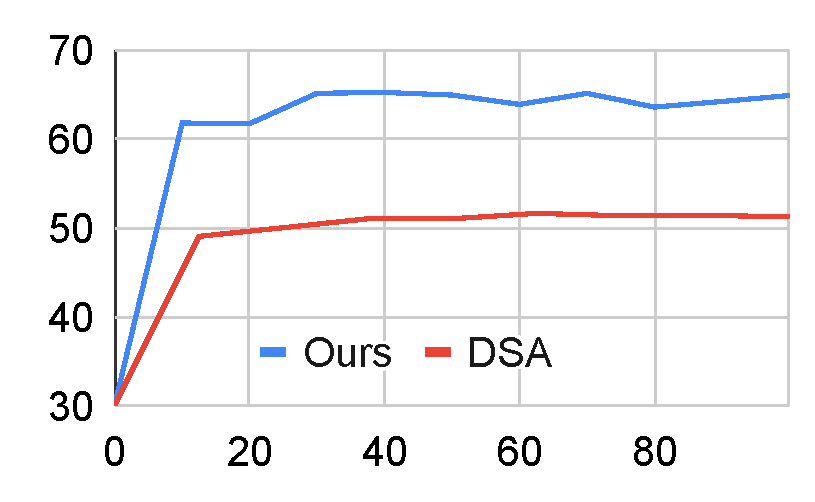
\includegraphics[trim={0.8cm 0.4cm 0.8cm 0.4cm},clip,align=c,width=0.4\linewidth]{figures/time.pdf}\\
&Distilling Time (mins)
\end{tabular}
}
\vspace{-8pt}
\caption{\textbf{Left}: ZCA Ablation. \textbf{Right}: Distillation Time.}
\vspace{-8pt}
\lblfig{zca}
\end{figure}

\subsubsection{Additional Ablation Studies}


\myparagraph{Initialization, normalization, and augmentation.}
In the main paper, we show ablations over several hyper-parameters. Here, we study the role of initialization, data normalization, and data augmentation for CIFAR-100 (1 image per class) in \reftbl{ablation}. For initialization in particular, recall that we typically initialize our synthetic images with real samples. Here, we evaluate initializing with Gaussian noise instead. Visualizations of these distilled sets can be seen in Figures \ref{fig:noise}-\ref{fig:noaug}. We also include a visualization of a set distilled with only one expert trajectory in \reffig{1exp}.

\begin{table}[!h]
    \centering
        \smaller
    \resizebox{\linewidth}{!}{
    \begin{tabular}{c|cccc}
       \toprule Setting  &  Ours & Gauss. Init. &  w/o ZCA & w/o Diff. Aug.\\
       \midrule Acc. & 24.3 $\pm$ 0.3 &  22.9 $\pm$ 0.4 & 19.1 $\pm$ 0.6 & 20.7 $\pm$ 0.7\\
       \bottomrule
    \end{tabular}
    }
    \caption{As we ablate our categorical hyper-parameters, we still achieve state-of-the-art performance (compared to \texttt{DSA}: 13.9\%). This is evaluated on CIFAR-100 with 1 image per class. Each design choice in our final method improves the performance of distilled images.  Here we use the default set of hyper-parameters for these ablations.}%
    \lbltbl{ablation}
\end{table}

\begin{figure}
\vspace{-4pt}
    \begingroup
    \setlength{\tabcolsep}{1pt}
    \centering
    \begin{tabular}{cccc}
        & \smaller{CIFAR-100 (1 Image / Class)} & & \smaller{CIFAR-100 (1 Image / Class)}\\
        \rotatebox[origin=c]{90}{\smaller{Validation Acc. \%}} &  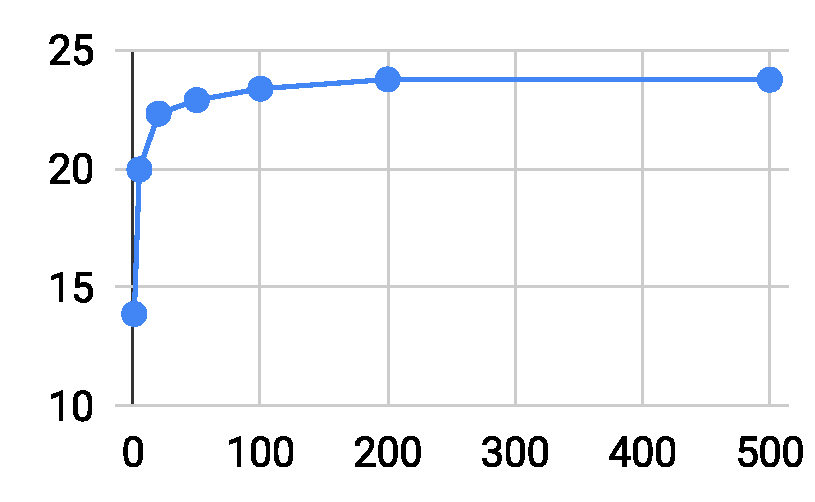
\includegraphics[align=c,width=0.43\linewidth]{figures/experts.pdf}& \hfill\;\;\;\;\rotatebox[origin=c]{90}{\smaller{Validation Acc. \%}} &  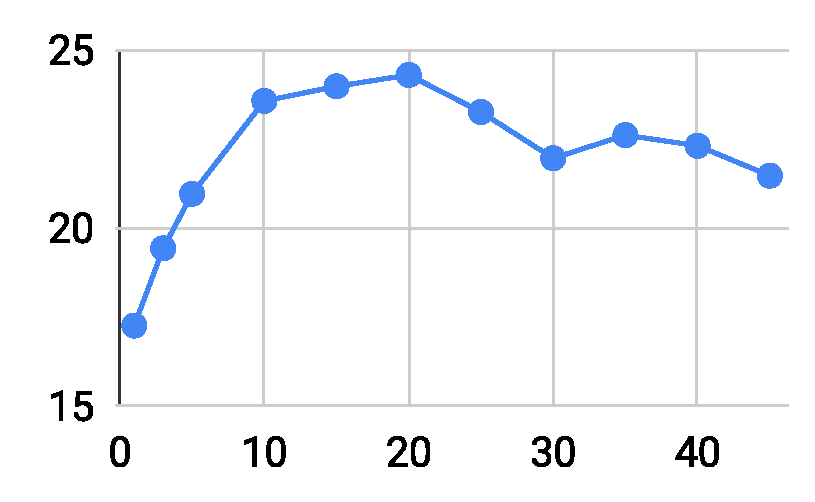
\includegraphics[align=c,width=0.43\linewidth]{figures/start-epoch.pdf}\\
         & \smaller{\;\;\;\;\;\# Expert Trajectories} & & \smaller{\;\;$T^+$: Max Start Epoch}
    \end{tabular}
    \endgroup
        \vspace{-7pt}
    \caption{\textbf{Left:} We see logarithmic performance improvement with respect to the number of expert trajectories used, quickly saturating near 200. \textbf{Right:} The upper bound on the expert epoch at which the synthetic data starts working cannot be too high or low to ensure quality learning signal.}
    \lblfig{experts}
    \vspace{-10pt}
\end{figure}

\begin{figure}
    \begingroup
    \setlength{\tabcolsep}{1pt}
    \centering
    \begin{tabular}{@{\hskip 0pt}cc@{\hskip 0pt}cc@{\hskip 0pt}}
    & \smaller{CIFAR-100 (1 Image / Class)} & & \smaller{CIFAR-100 (1 Image / Class)}\\
         \rotatebox[origin=c]{90}{\fontsize{6}{5}\selectfont{$\alpha$: Learned Step Size}} &  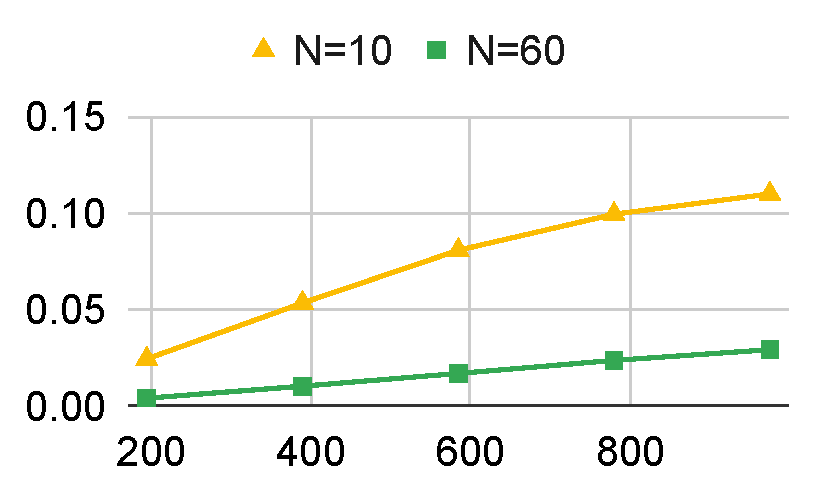
\includegraphics[align=c,width=0.455\linewidth]{figures/learningrate.pdf}& \hfill\;\;\rotatebox[origin=c]{90}{\fontsize{6}{5}\selectfont{Validation Acc. \%}} &  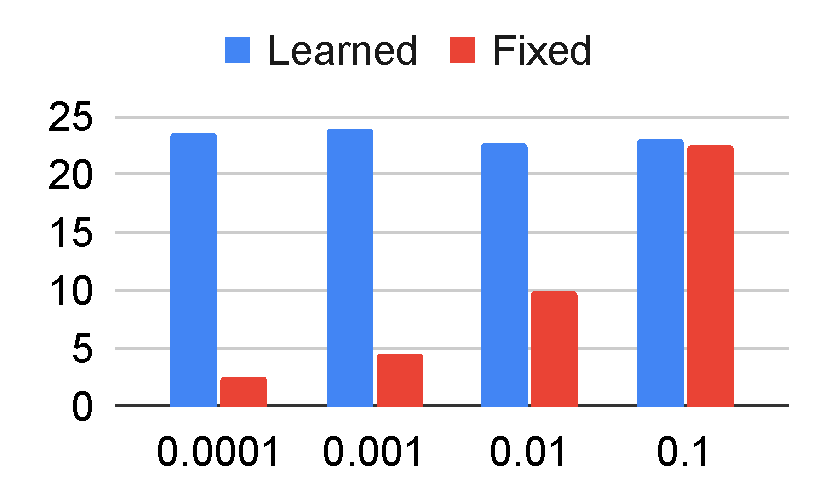
\includegraphics[align=c,width=0.458\linewidth]{figures/lr_lr.pdf}\\[-1.3ex]
         & \fontsize{6}{5}\selectfont{\;\;\;\;\;$M$: Expert Steps} & & \fontsize{6}{5}\selectfont{\;\;$\alpha_0$: Initial Synthetic Step Size}
    \end{tabular}
    \endgroup
        \vspace{-9pt}
    \caption{\textbf{Left:} Our learned synthetic step size $\alpha$ seems to scale inversely with the number of synthetic steps $N$ to cover the same distance in parameter space as the expert steps $M$.
    \textbf{Right:} Having a learnable step size $\alpha$ saves us from having to search for an appropriate fixed $\alpha_0$.
    }
    \lblfig{lr}
    \vspace{-10pt}
\end{figure}

\myparagraph{Performance w.r.t. the number of expert trajectories.}
Since they effectively make up our method's ``training set,'' it is reasonable to assume that having more expert trajectories would lead to better performance. We see that this is indeed the case for the CIFAR-100, 1 image per class setting in \reffig{experts} (left). However, what's most interesting is the sharp, logarithmic increase in validation accuracy w.r.t. the number of experts. We note the most amount of improvement when increasing from  1 to 20 experts but see almost complete saturation by the time we reach 200. Given how high-dimensional the parameter space of a neural network is, it is remarkable that we can achieve such high performance with so few expert trajectories. \vspace{10pt}

\myparagraph{Performance w.r.t. expert time-step range.}
When we initialize our student networks, we do so at a randomly selected time-step from an expert trajectory. We find that it is important to put an upper bound on this starting time-step (\reffig{experts}, right). If the upper bound is too high, the synthetic data receives gradients from points where the experts movements are small and uninformative. If it is too low, the synthetic data is never exposed to mid and later points in the trajectories, missing out on a significant portion of the training dynamics.


\begin{figure}
    \centering
    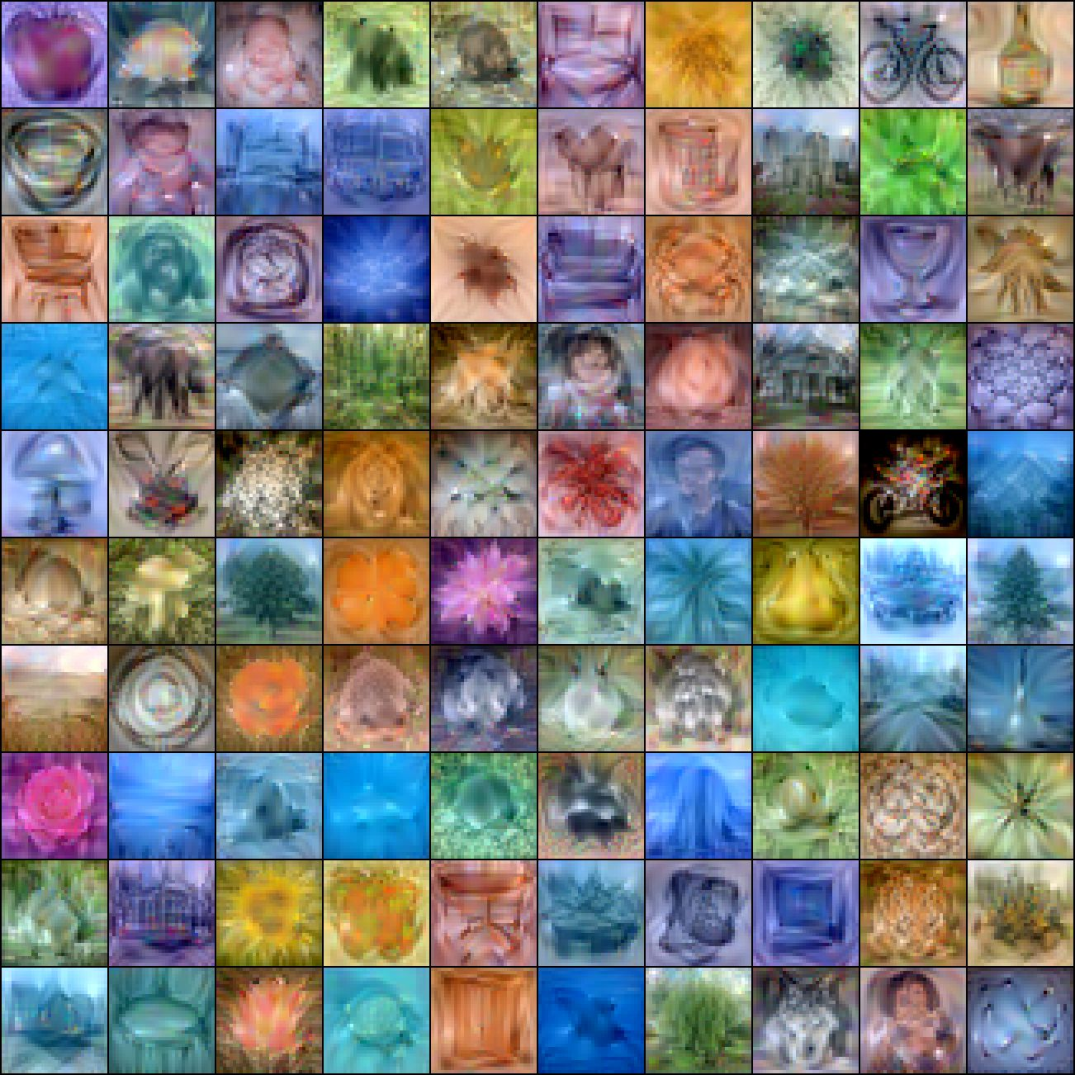
\includegraphics[width=\linewidth]{figures/CIFAR100.pdf}
    \caption{CIFAR-100, 1 Image Per Class}
    \lblfig{cifar-100}
    \vspace{-9pt}
\end{figure}

\subsection{Experiment Details}
\myparagraph{Hyper-Parameters.}
In \reftbl{hparams}, we enumerate the hyper-parameters used for our results reported in the main text. Limited compute forced us to batch our synthetic data for some of the larger sets. The ``ConvNet'' architectures are as explained in the main text.
\begin{table}
\renewcommand\arraystretch{0.9}
\centering
\scriptsize
\setlength{\tabcolsep}{2pt}
\resizebox{0.98\linewidth}{!}{
\begin{tabular}{ccc|ccccc}
\toprule
Dataset         & Model & Img/Cls & \makecell{Synthetic \\ Steps \\ ($N$)} & \makecell{Expert \\ Epochs \\($M^\dagger$)}  & \makecell{Max Start \\ Epoch \\ ($T^+$)}  & \makecell{Synthetic \\ Batch Size \\ ($|b|$)} & ZCA \\ \midrule


\multirow{3}{*}{CIFAR-10}  & \multirow{3}{*}{ConvNetD3}      & 1   & 50   & 2  & 2 & - & Y\\
                               & & 10  & 30    & 2  & 20 & - & Y\\
                               & & 50  & 30      & 2 & 40  &  -  & N\\ \midrule
                                
\multirow{3}{*}{CIFAR-100} & \multirow{3}{*}{ConvNetD3}     & 1   & 20   & 3  &  20  & - & Y \\ 
                              && 10  & 20      & 2  & 20  & - & N\\  
                              && 50  & 80     & 2  & 40  & -   & Y     \\  \midrule

\multirow{3}{*}{Tiny ImageNet} & \multirow{3}{*}{ConvNetD4} & 1   & 10    &  2  &  10  &  - & -\\ 
                             & & 10  & 20      &  2  & 40  &  200 & -  \\  
                             & & 50  & 20     & 2  & 40  & 300  & -\\  \midrule
                              
\multirow{2}{*}{ImageNet (All)} & \multirow{2}{*}{ConvNetD5} & 1   & 20    &  2  &  10  &  - & -\\ 
                             & & 10  & 20      &  2  & 10  &  20  & - \\  \bottomrule

\end{tabular}
}
\caption{Hyper-parameters used for our best-performing distillation experiments. A synthetic batch size of ``-'' indicates that we used the full support set at each synthetic step. Note: instead of number of expert \textit{updates} ($M$), here we list number of expert \textit{epochs} ($M^\dagger$) for simplicity across datasets.}
\lbltbl{hparams}
     \vspace{-6pt}
\end{table}




\myparagraph{Compute resources.} We had a relatively limited compute budget for our experiments, using any GPU we could access. As such, our experiments were run on a mixture of RTX2080ti, RTX3090, and RTX6000 GPUs. The largest amount of VRAM we used for a single experiment was 144GB over 6xRTX6000 GPUs.

\myparagraph{Training Time.} Distillation time varied based on dataset and type and number of GPUs used. Regardless of dataset or compute resources, time per distillation iteration scaled linearly with the number of synthetic steps $N$. For CIFAR-100, 1 image per class with $N=20$, we had an average time of 0.6 seconds per distillation step when using a single RTX3090. We ran our experiments for 10000 distillation steps but saw the most improvement within the first 1000.

Our distillation time, in general, is comparable to \texttt{DC/DSA}, as they also utilize a bi-level optimization. In the 10 img/class setting (for example), \texttt{DC/DSA} trains on the synthetic data for 50 epochs on the between each update. We include a sample distillation curve in \reffig{zca} (Right). Both experiments were run on RTX3090. Note that  \texttt{KIP} requires over 1,000 GPU hours.

Regarding the distillation time for learning different sets on CIFAR10/100 and TinyImageNet, we report them in \reftbl{time}. Note that most improvement occurs within the first 1k iterations, but we continue training for 10k.
\begin{table}[!h]
\renewcommand\arraystretch{0.9}
\centering
\scriptsize
\setlength{\tabcolsep}{2pt}
\resizebox{0.75\linewidth}{!}{
\begin{tabular}{cc|c|ccc}
\toprule
        Dataset & Img/Cls  & \makecell{1 Iter.\\(sec)} & \makecell{1k Iter.\\(min)} & \makecell{5k Iter.\\(min)} & \makecell{10k Iter.\\(min)}\\ \midrule  %


\multirow{3}{*}{CIFAR-10}        & 1      & 0.5 & 8 & 42 & 83\\
                                & 10     & 0.6 & 10 & 50 & 100\\  
                                & 50       & 0.8 & 13 & 67 & 133\\ \midrule
                                
\multirow{3}{*}{CIFAR-100}     & 1      &  0.6 & 10 &50 & 100\\ 
                              & 10       & 0.8 & 13 & 67 & 133\\  
                              & 50       & 1.9 & 32 & 158 & 317\\  \midrule

\multirow{3}{*}{Tiny ImageNet} & 1       &  1.1 & 18 & 92 & 183\\ 
                              & 10      &  2.3 & 38 & 192 & 383\\  
                              & 50      & 2.6 & 43 & 217 & 433\\  \bottomrule


\end{tabular}
}
\vspace{-8pt}
\caption{Distillation time for each dataset and support size.}
\lbltbl{time}
\end{table}




\myparagraph{KIP to NN}
In the \texttt{KIP} paper, results are presented for images distilled using the neural tangent kernel method and then evaluated by training a modified width-1024 ConvNetD3. Aside from the increased width of the finite model, the ConvNet architecture used in the \texttt{KIP} paper also has an additional 1-layer convolutional stem.

Using the training notebook provided with the \texttt{KIP} paper, we perform an exhaustive search over a reasonable set of hyper-parameters for the KIP to width-128 NN problem: \texttt{checkpoint} $\in$ \{112, 335, 1000\}, \texttt{weight\_decay} $\in $ \{0, 0.0001, 0.001, 0.01\}, \texttt{aug} $\in$ \{\texttt{True}, \texttt{False}\}, \texttt{zca} $\in$ \{\texttt{True}, \texttt{False}\}, \texttt{label\_learn} $\in$ \{\texttt{True}, \texttt{False}\}, and \texttt{norm} $\in$ \{\texttt{none}, \texttt{instance}\}. The architecture originally used for KIP to NN in the \texttt{KIP} paper contained no normalization layers. However, we found that with the smaller width, this model could not even converge on the synthetic training data for CIFAR-100, so we added instance normalization layers as found in the ConvNets we and \texttt{DC}, \texttt{DSA}, and \texttt{DM} use.

In \reftbl{kip_hyperparams}, we include the optimal hyper-parameters from this search that were used to obtain the KIP to NN (128\nobreakdash-width) values reported in the main text.


\begin{table}
\centering\vspace{-8pt}
\resizebox{0.95\linewidth}{!}{
\begin{tabular}{cc|cccccc}
\toprule
 & Img/Cls  & \makecell{Learn\\Labels} & Aug. & ZCA & Norm & \makecell{Weight\\Decay} & Ckpt.\\ \midrule 
\multirow{3}{*}{CIFAR-10}  & 1  & N & Y & Y & N & 0.001 & 1000\\
                          & 10  & N &  N & Y & N & 0.001 & 112\\
                          & 50  & N & N & Y & I & 0.01 & 112\\ \midrule
\multirow{2}{*}{CIFAR-100} & 1   & N & N & Y & I & 0.001 & 1000\\
                          & 10  & N & N & N & I & 0.001 & 1000\\
\bottomrule
\end{tabular}
}
\caption{Optimal hyper-parameters for our reported width-128 KIP to NN results. These were obtained via grid search using the notebook provided by the KIP authors.}
\lbltbl{kip_hyperparams}
\vspace{-8pt}
\end{table}









\begin{figure}
    \centering
    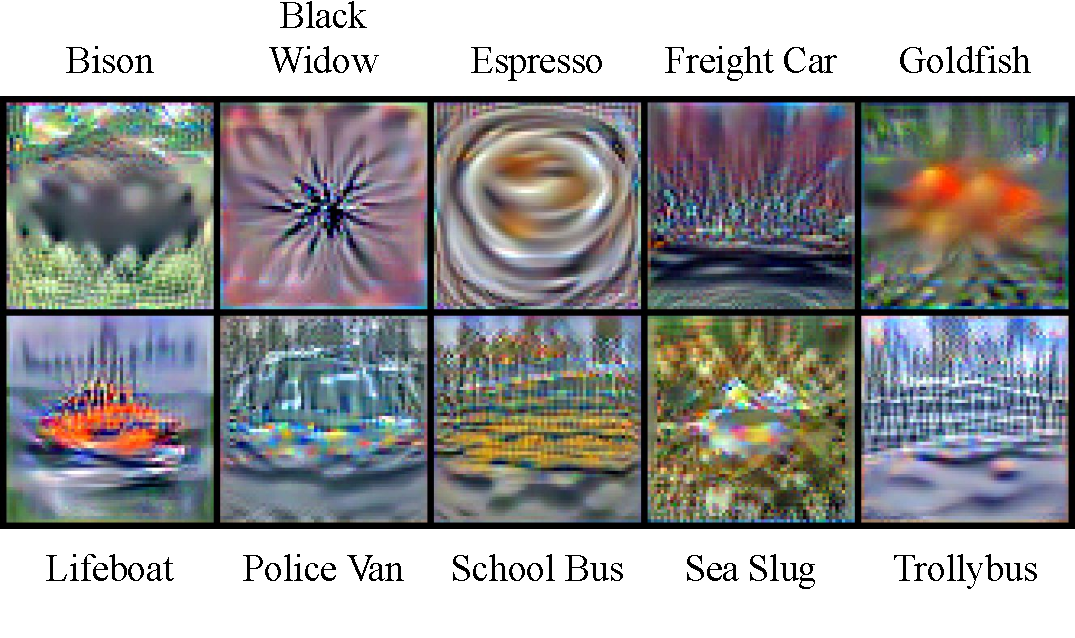
\includegraphics[width=\linewidth]{figures/Tiny_Good.pdf}
    \vspace{-20pt}
    \caption{Most-correct distilled images for Tiny ImageNet \smaller{($\geq 30\%$)}}
    \label{fig:tinygood}
    \vspace{-8pt}
\end{figure}
\begin{figure}
    \centering
    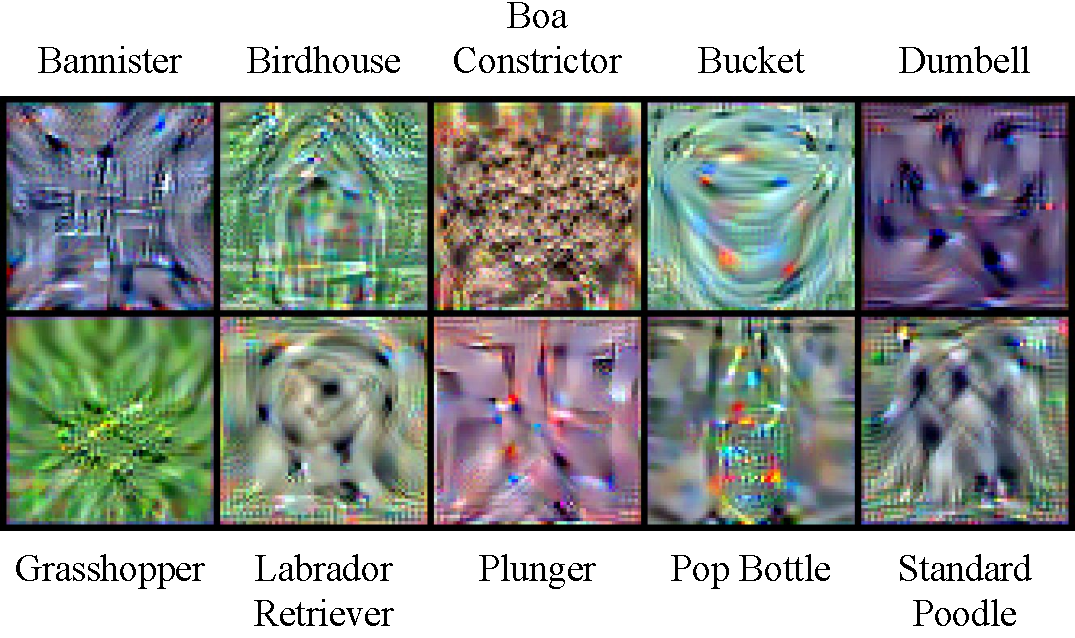
\includegraphics[width=\linewidth]{figures/Tiny_Bad.pdf}
    \vspace{-8pt}
    \caption{Least-correct distilled images for Tiny ImageNet \smaller{($\leq 4\%$)}}
    \label{fig:tinybad}
    \vspace{-8pt}
\end{figure}


\clearpage

\begin{figure}
    \centering
    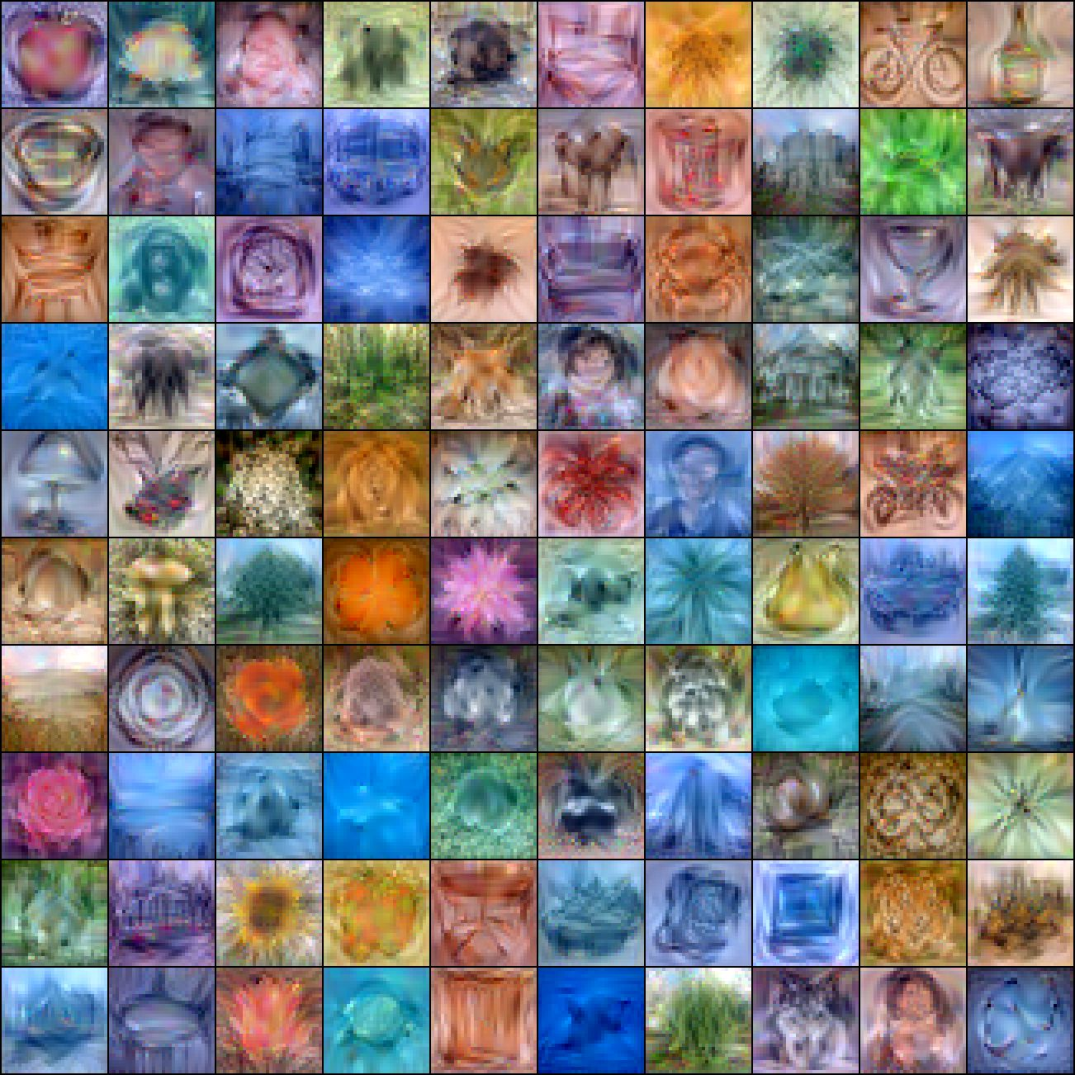
\includegraphics[width=\linewidth]{figures/cifar100-noise.pdf}
    \caption{CIFAR-100, Initialized as Random Noise}
    \label{fig:noise}
\end{figure}
\begin{figure}
    \centering
    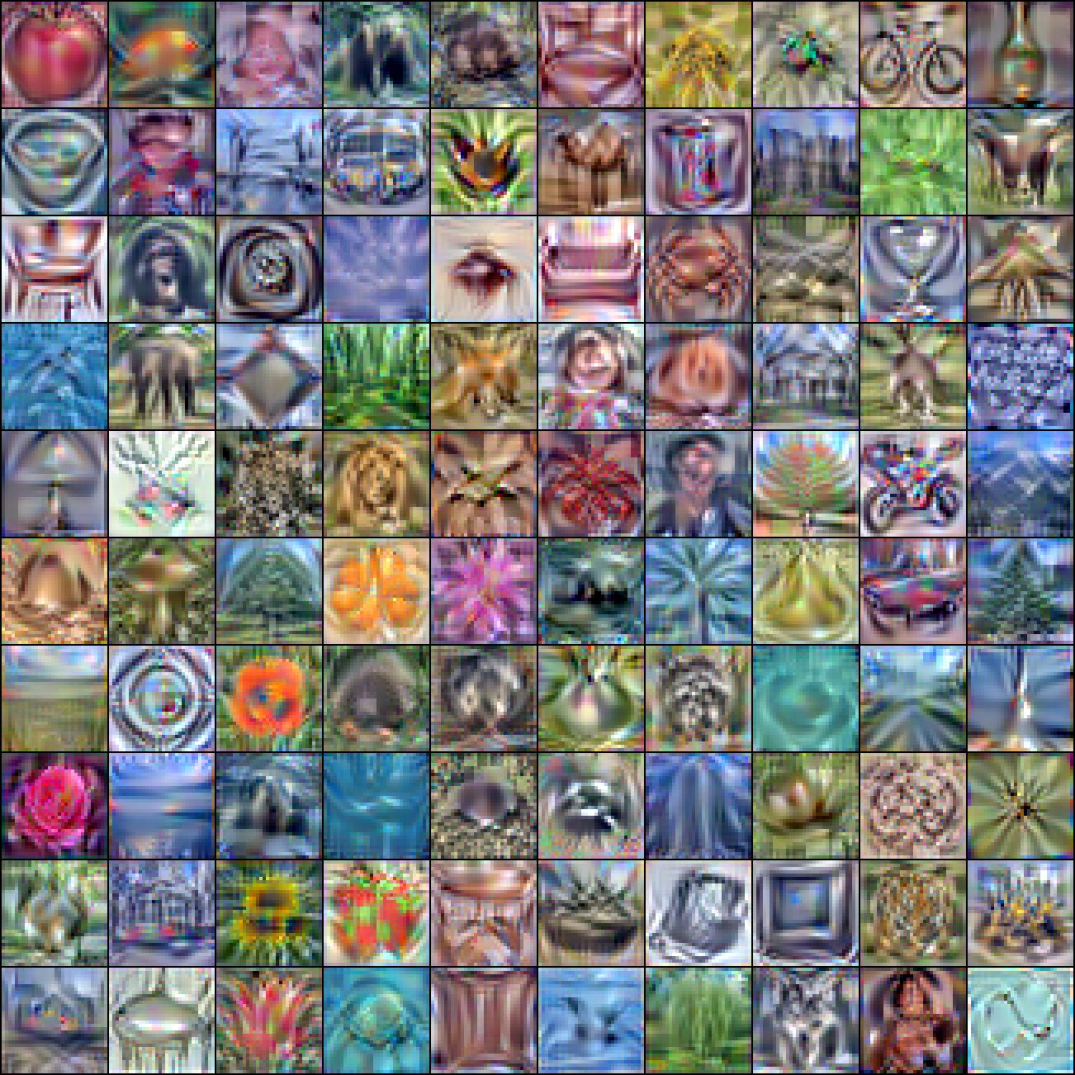
\includegraphics[width=\linewidth]{figures/cifar100-nozca.pdf}
    \caption{CIFAR-100, No ZCA Whitening}
    \label{fig:nozca}
\end{figure}
\begin{figure}
    \centering
    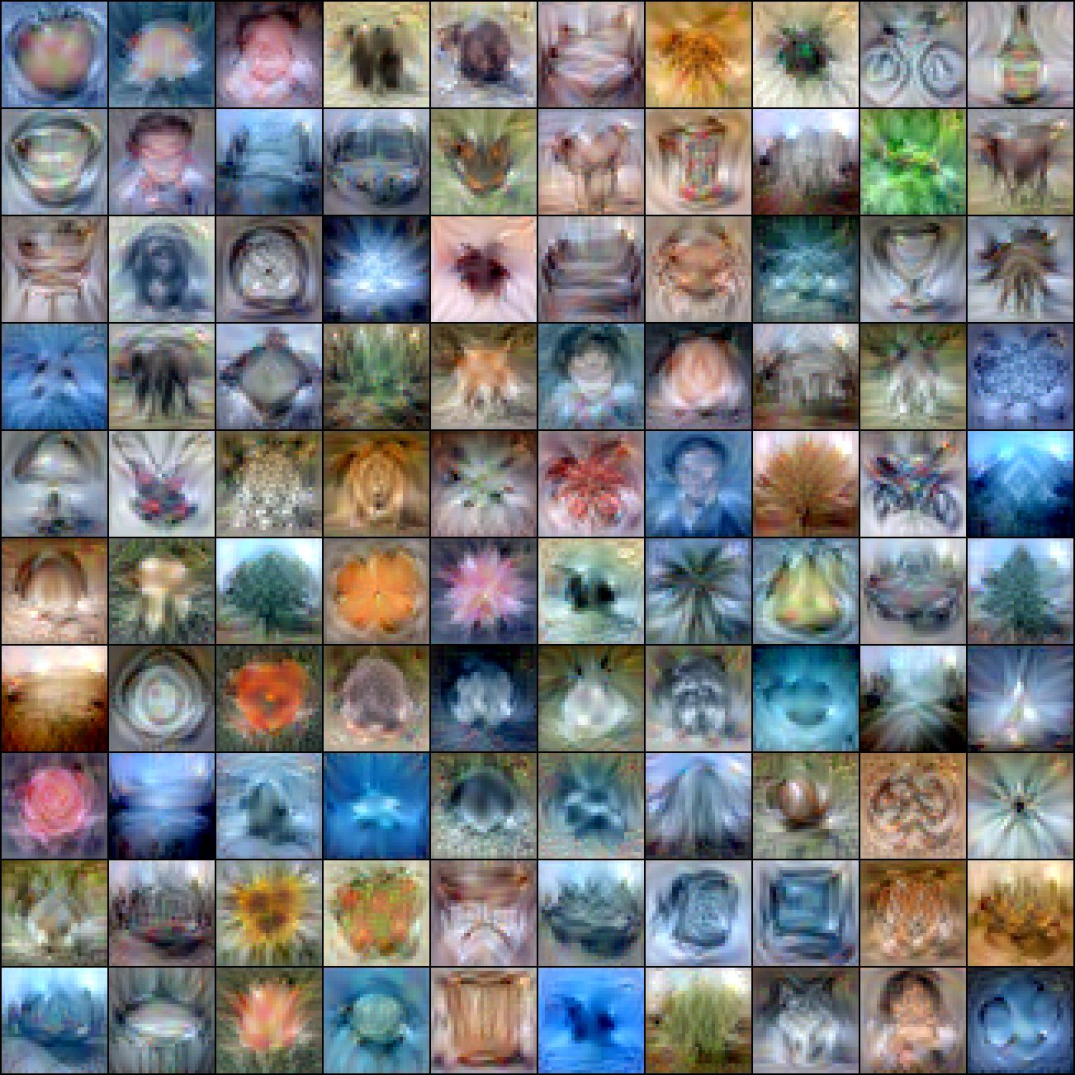
\includegraphics[width=\linewidth]{figures/cifar100-noaug.pdf}
    \caption{CIFAR-100, No Differentiable Augmentation}
    \label{fig:noaug}
\end{figure}
\begin{figure}
    \centering
    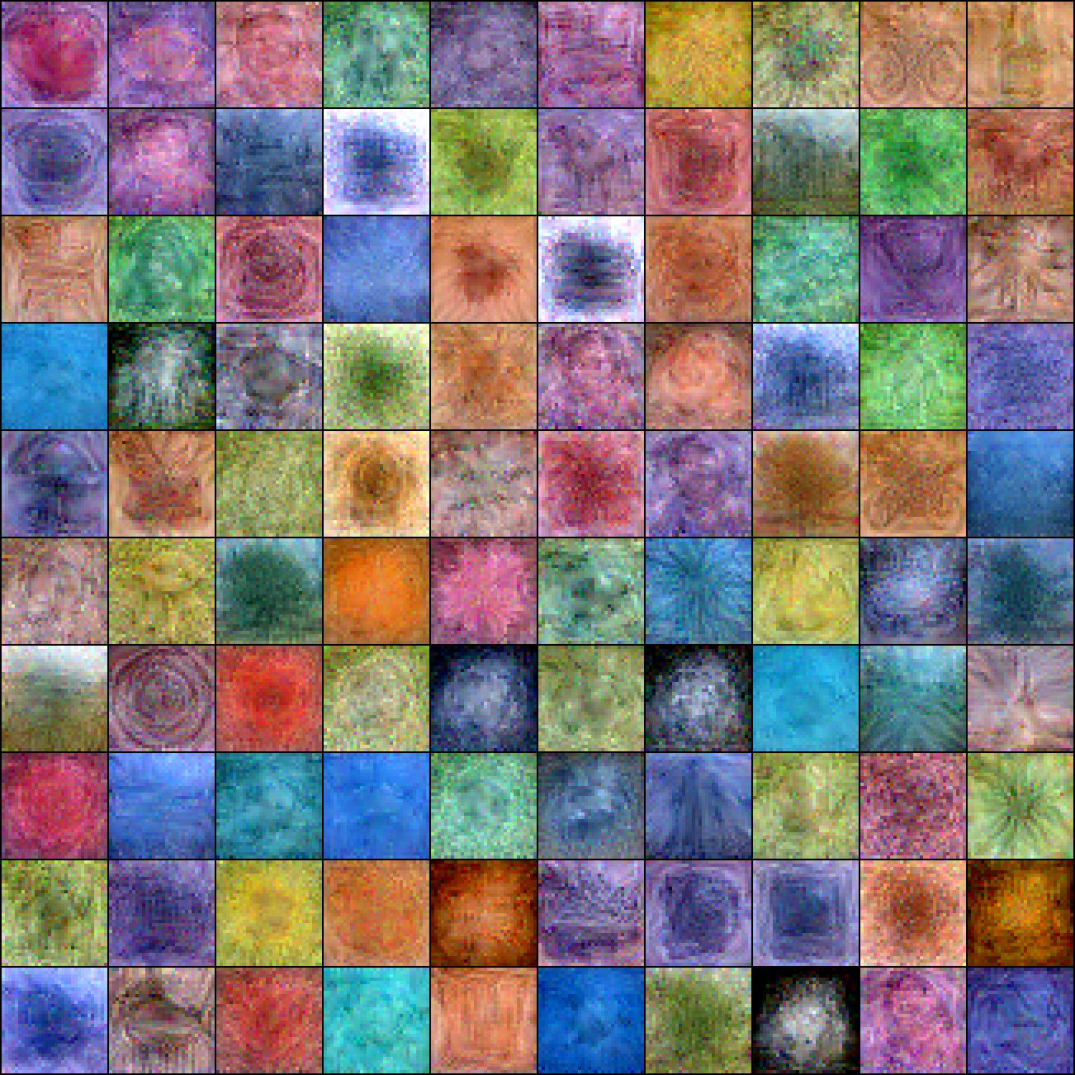
\includegraphics[width=\linewidth]{figures/cifar100-single.pdf}
    \caption{CIFAR-100, Only 1 Expert Trajectory}
    \label{fig:1exp}
\end{figure}

\begin{figure*}
    \centering
    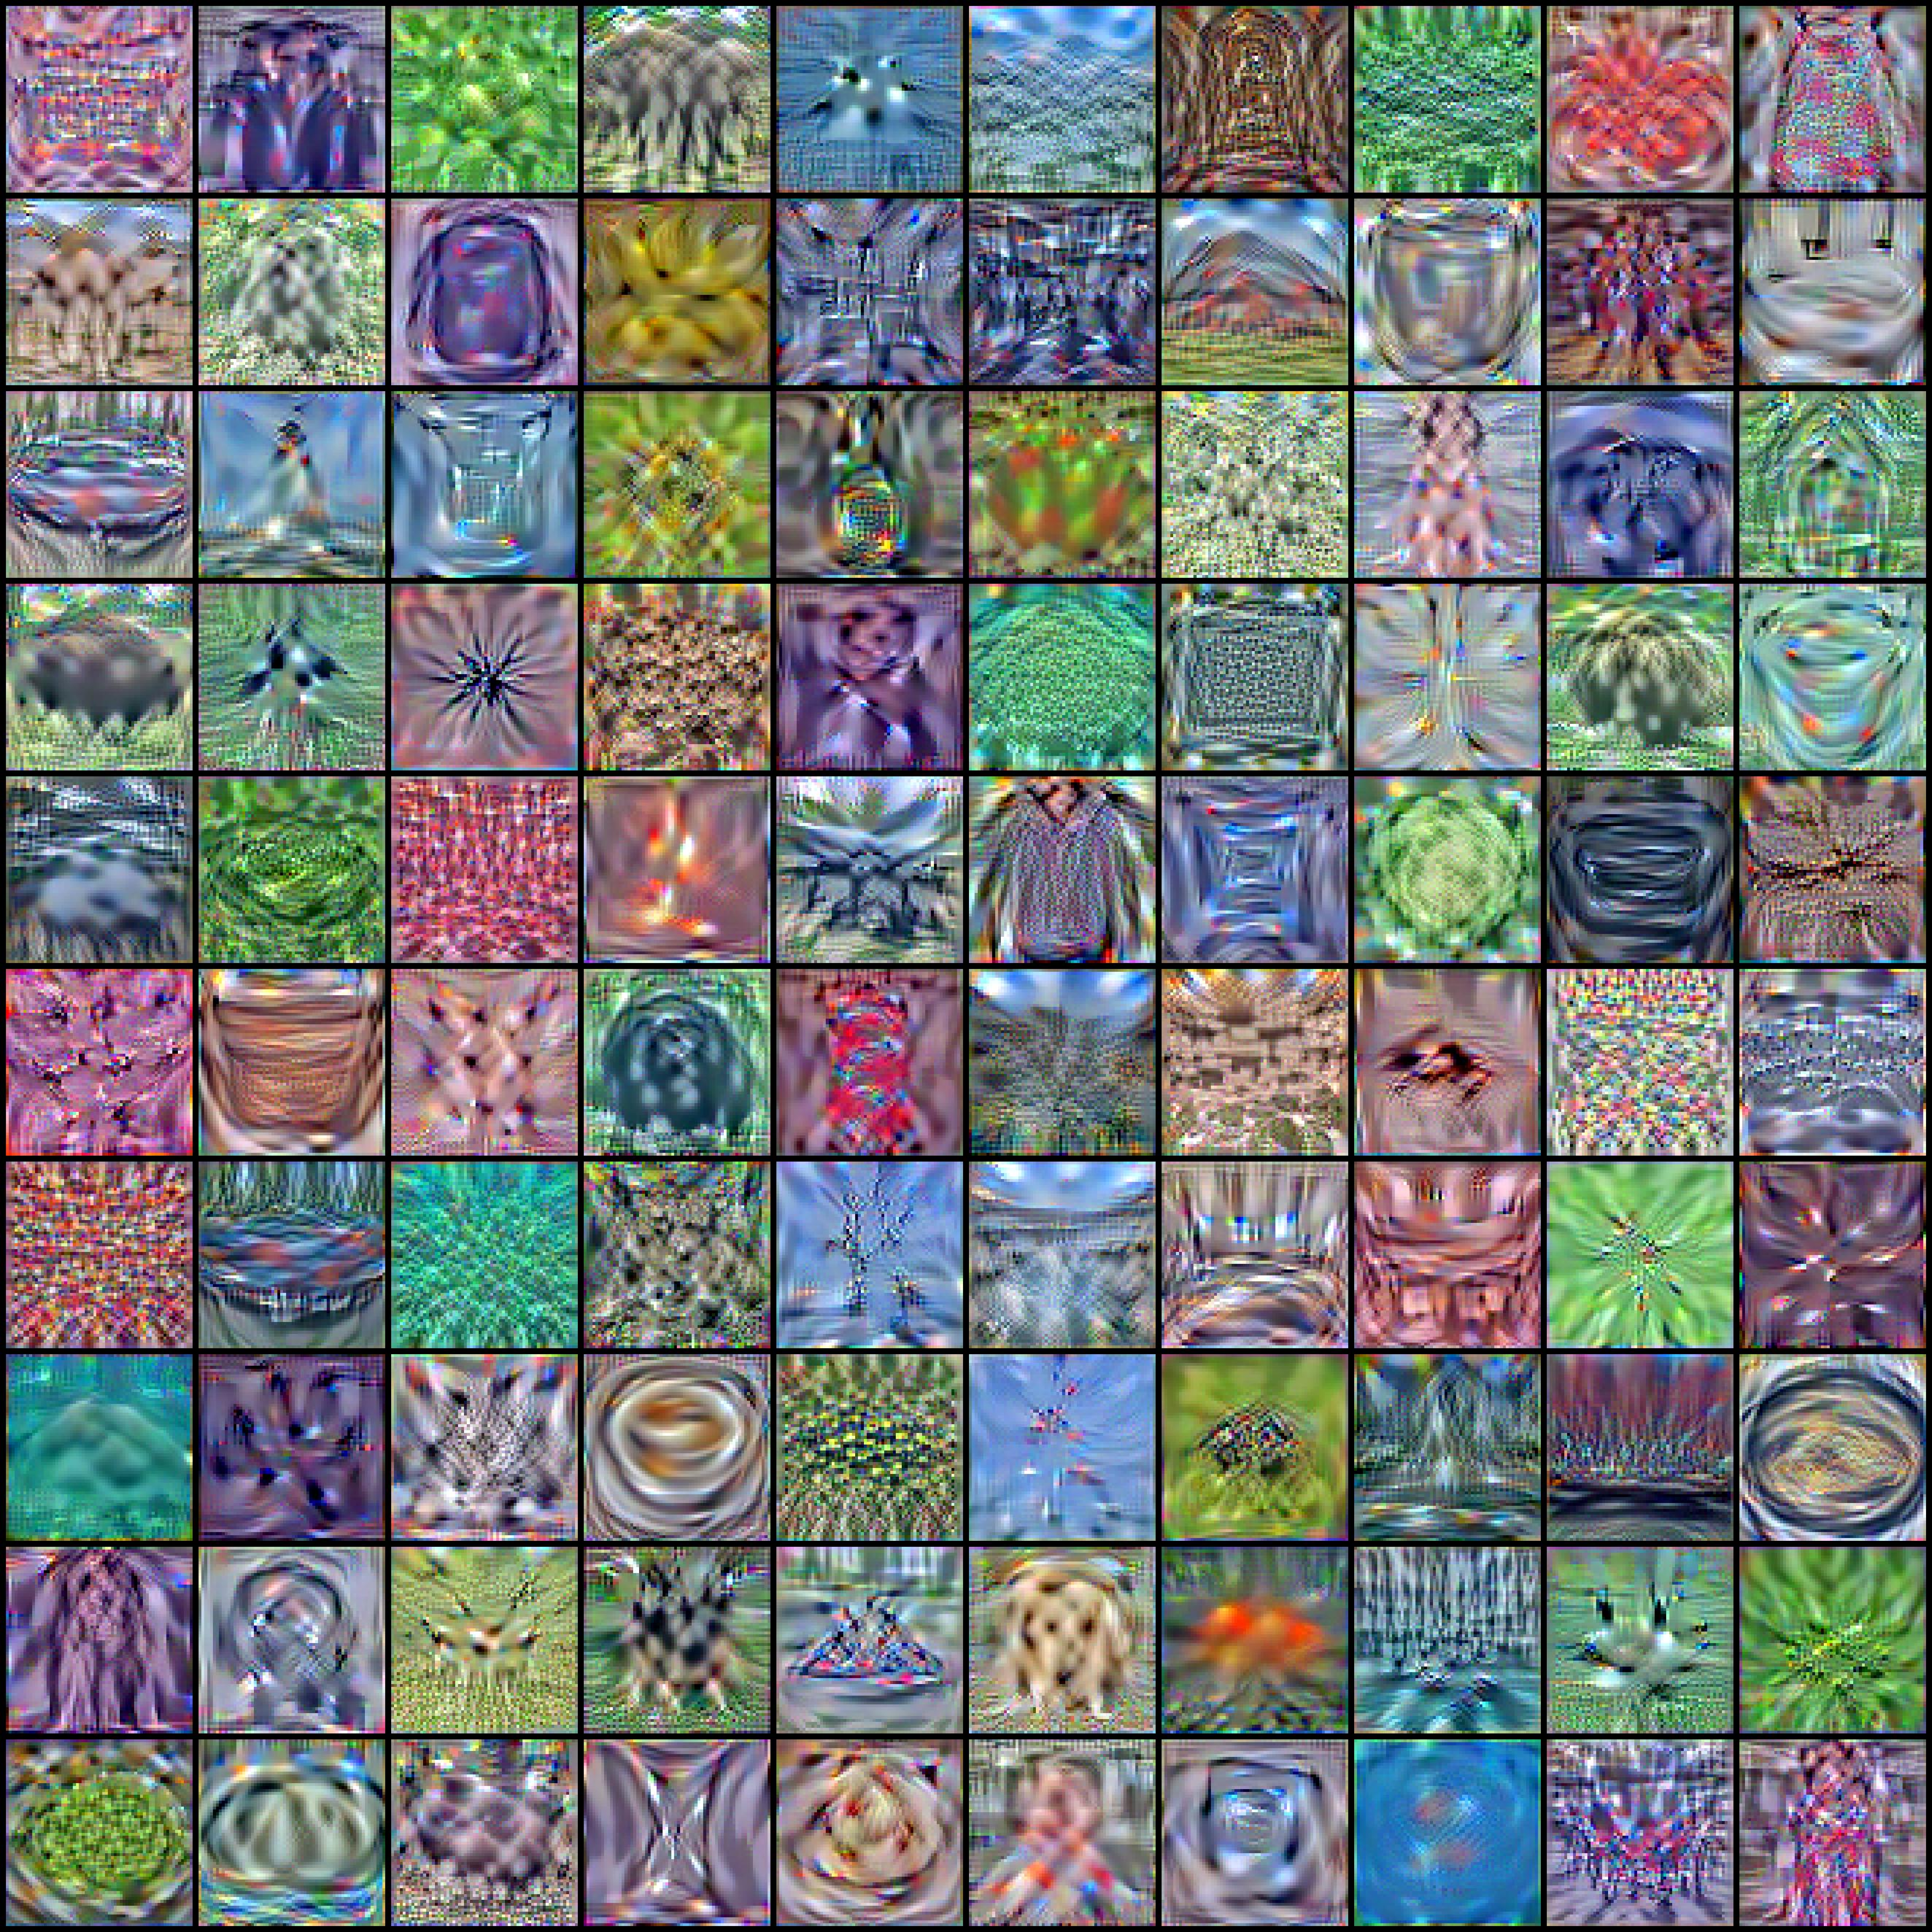
\includegraphics[width=\linewidth]{figures/tiny_all_1.pdf}
    \caption{Tiny ImageNet, 1 Image Per Class (Classes 1-100)}
    \label{fig:tiny1}
\end{figure*}

\begin{figure*}
    \centering
    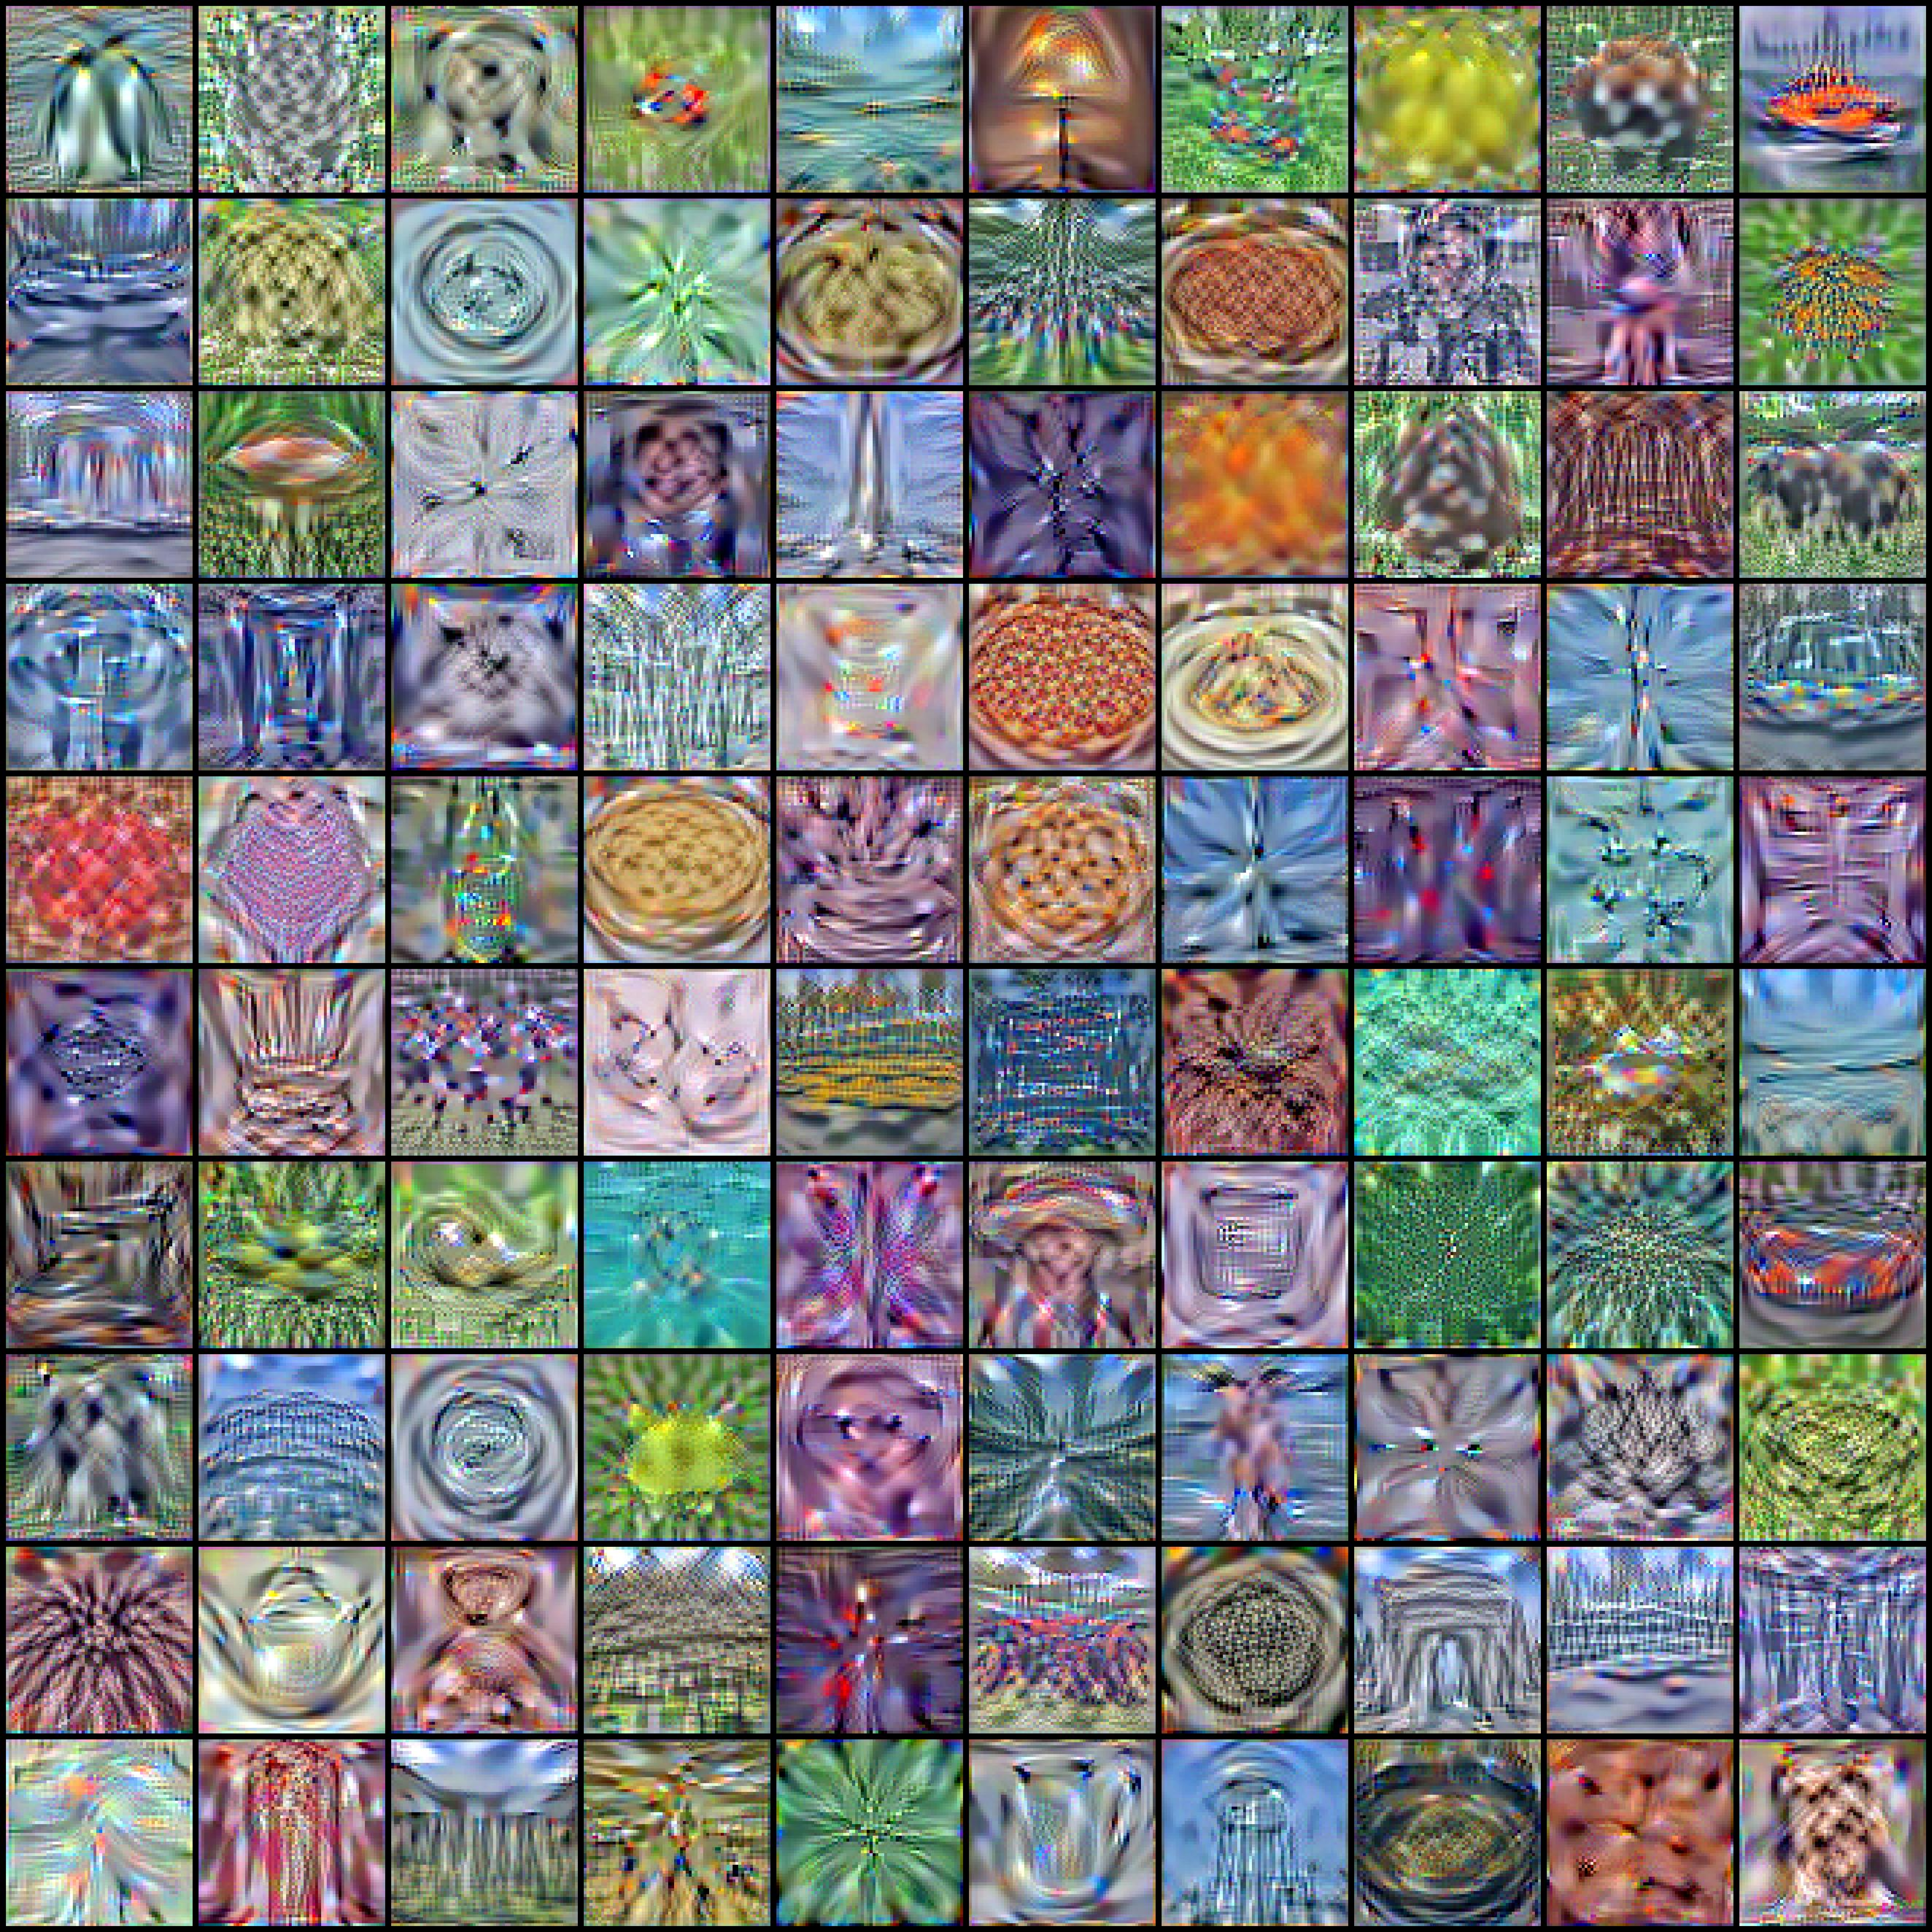
\includegraphics[width=\linewidth]{figures/tiny_all_2.pdf}
    \caption{Tiny ImageNet, 1 Image Per Class (Classes 101-200)}
    \label{fig:tiny2}
\end{figure*}

\begin{figure*}
    \centering
    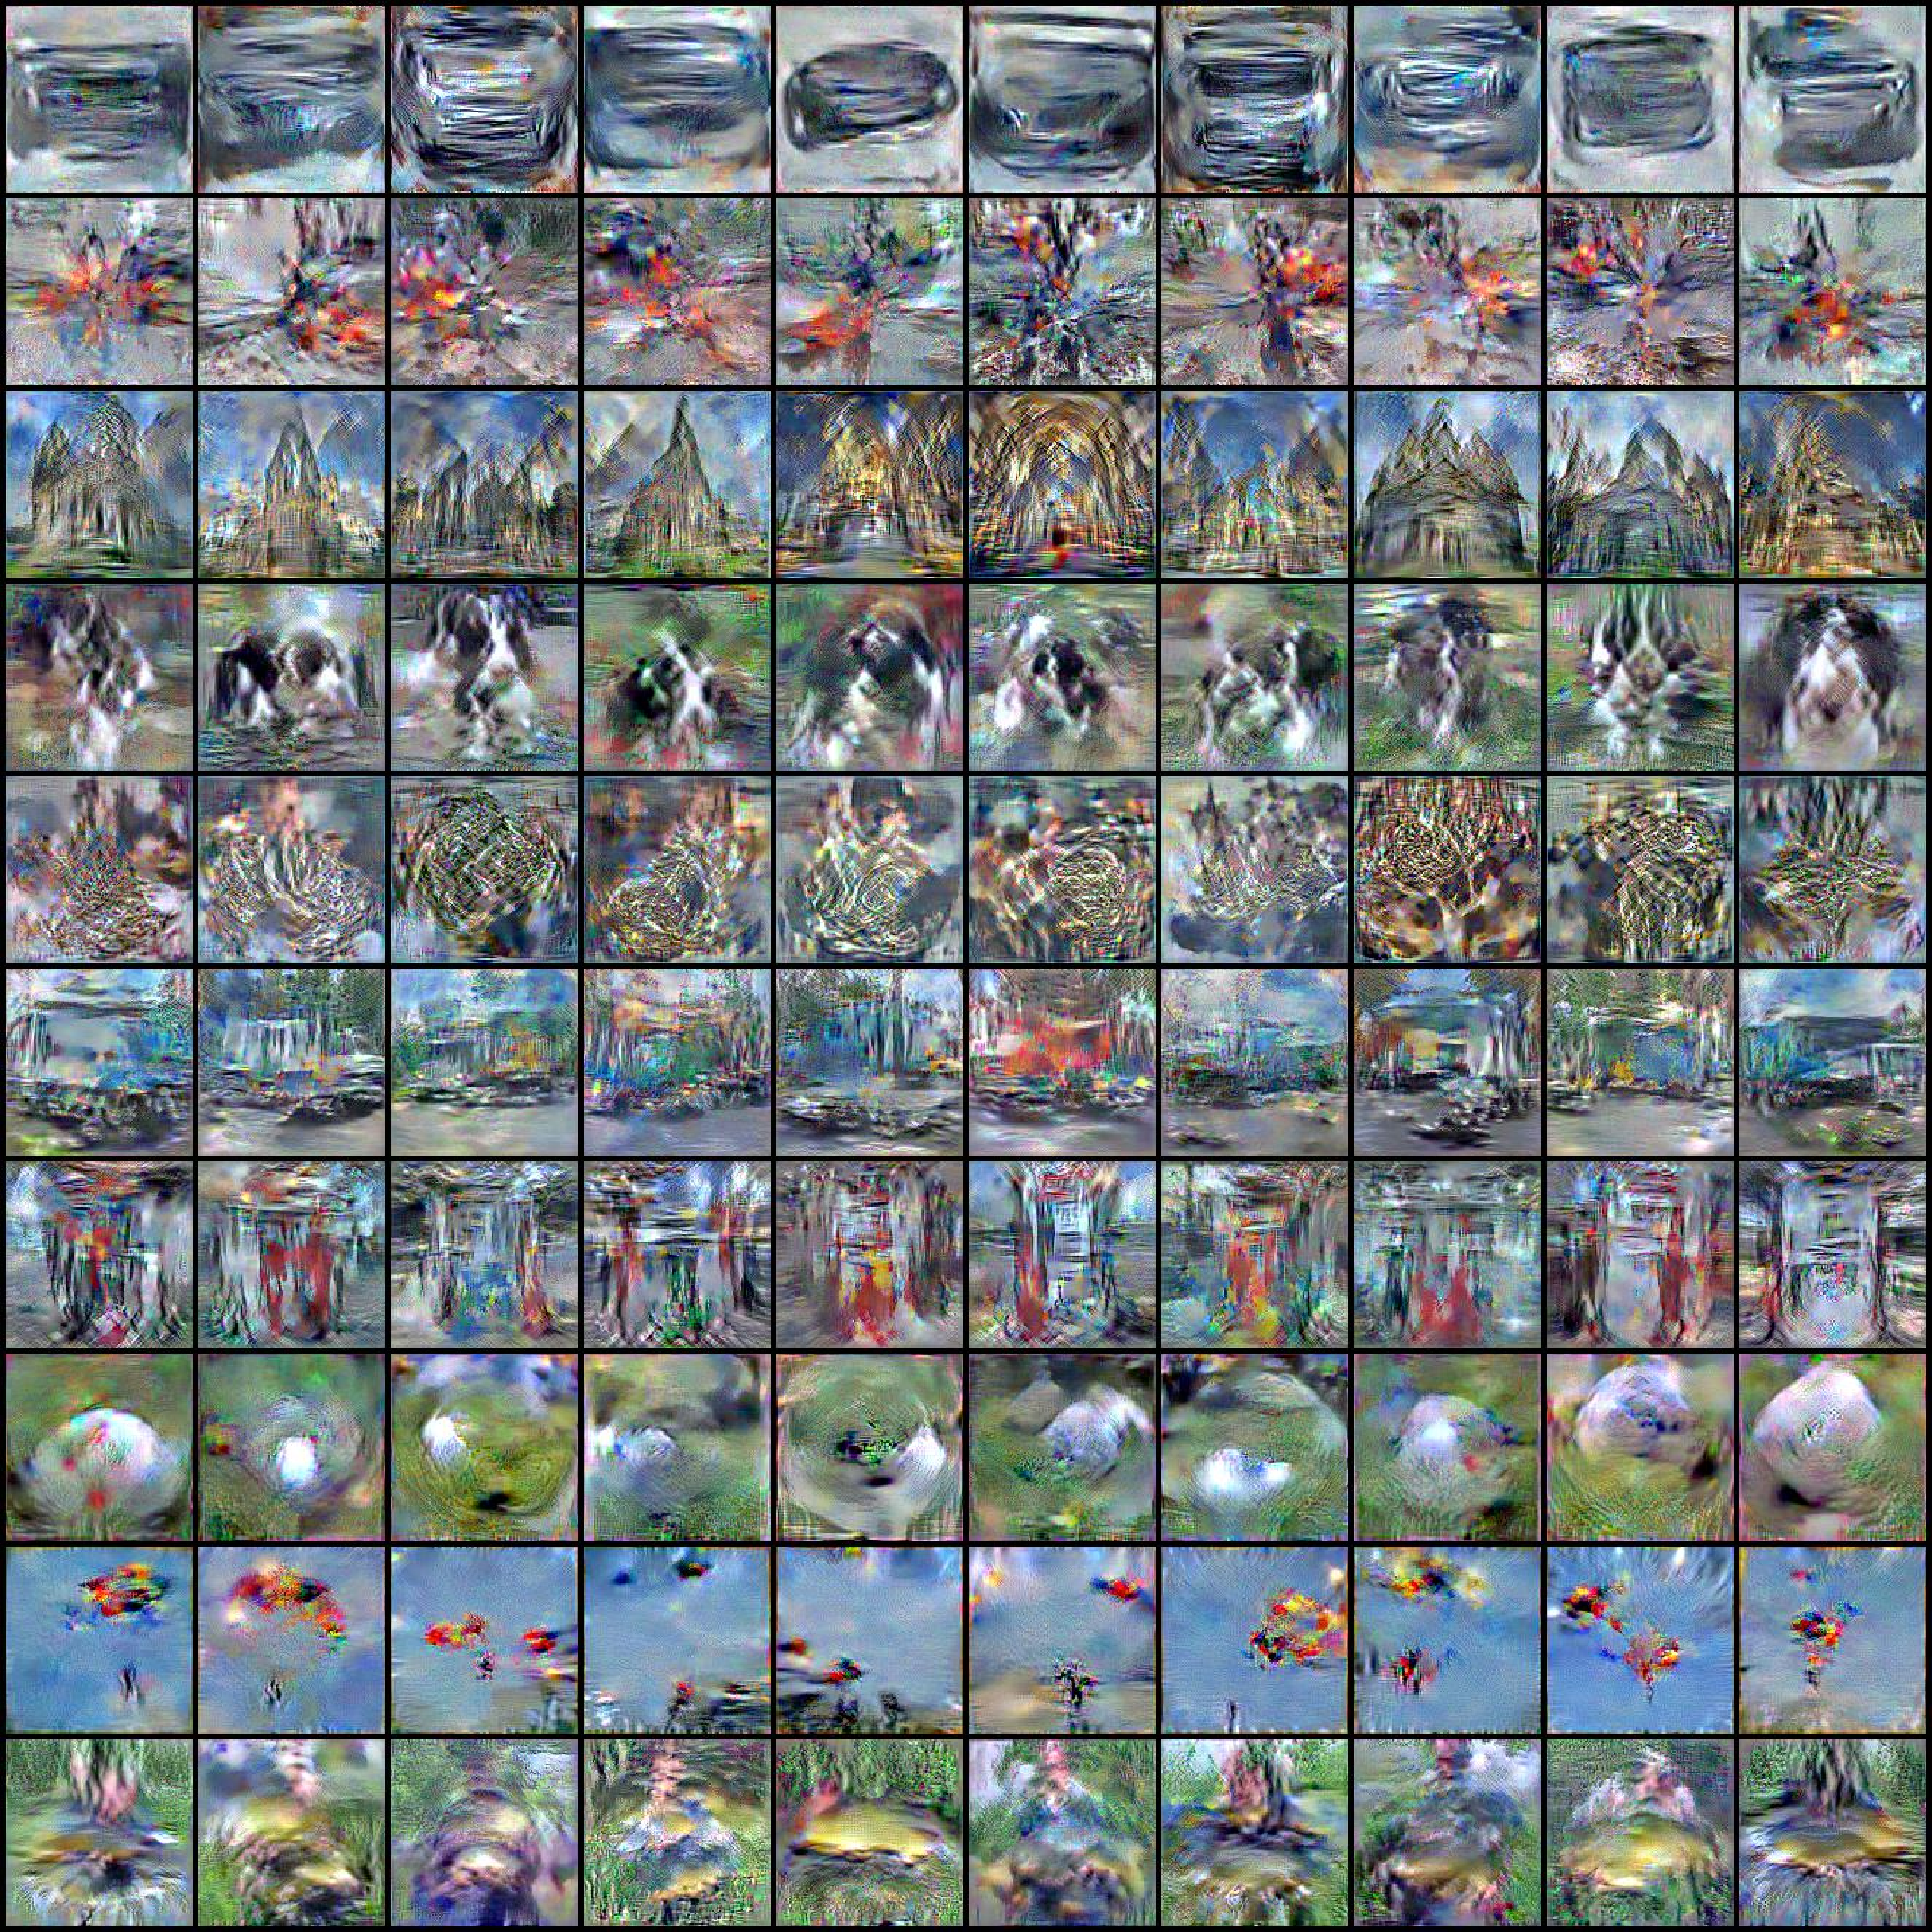
\includegraphics[width=\linewidth]{figures/imagenet_10/imagenette_all.pdf}
    \caption{ImageNette, 10 Images Per Class}
    \label{fig:nette_10}
\end{figure*}
\begin{figure*}
    \centering
    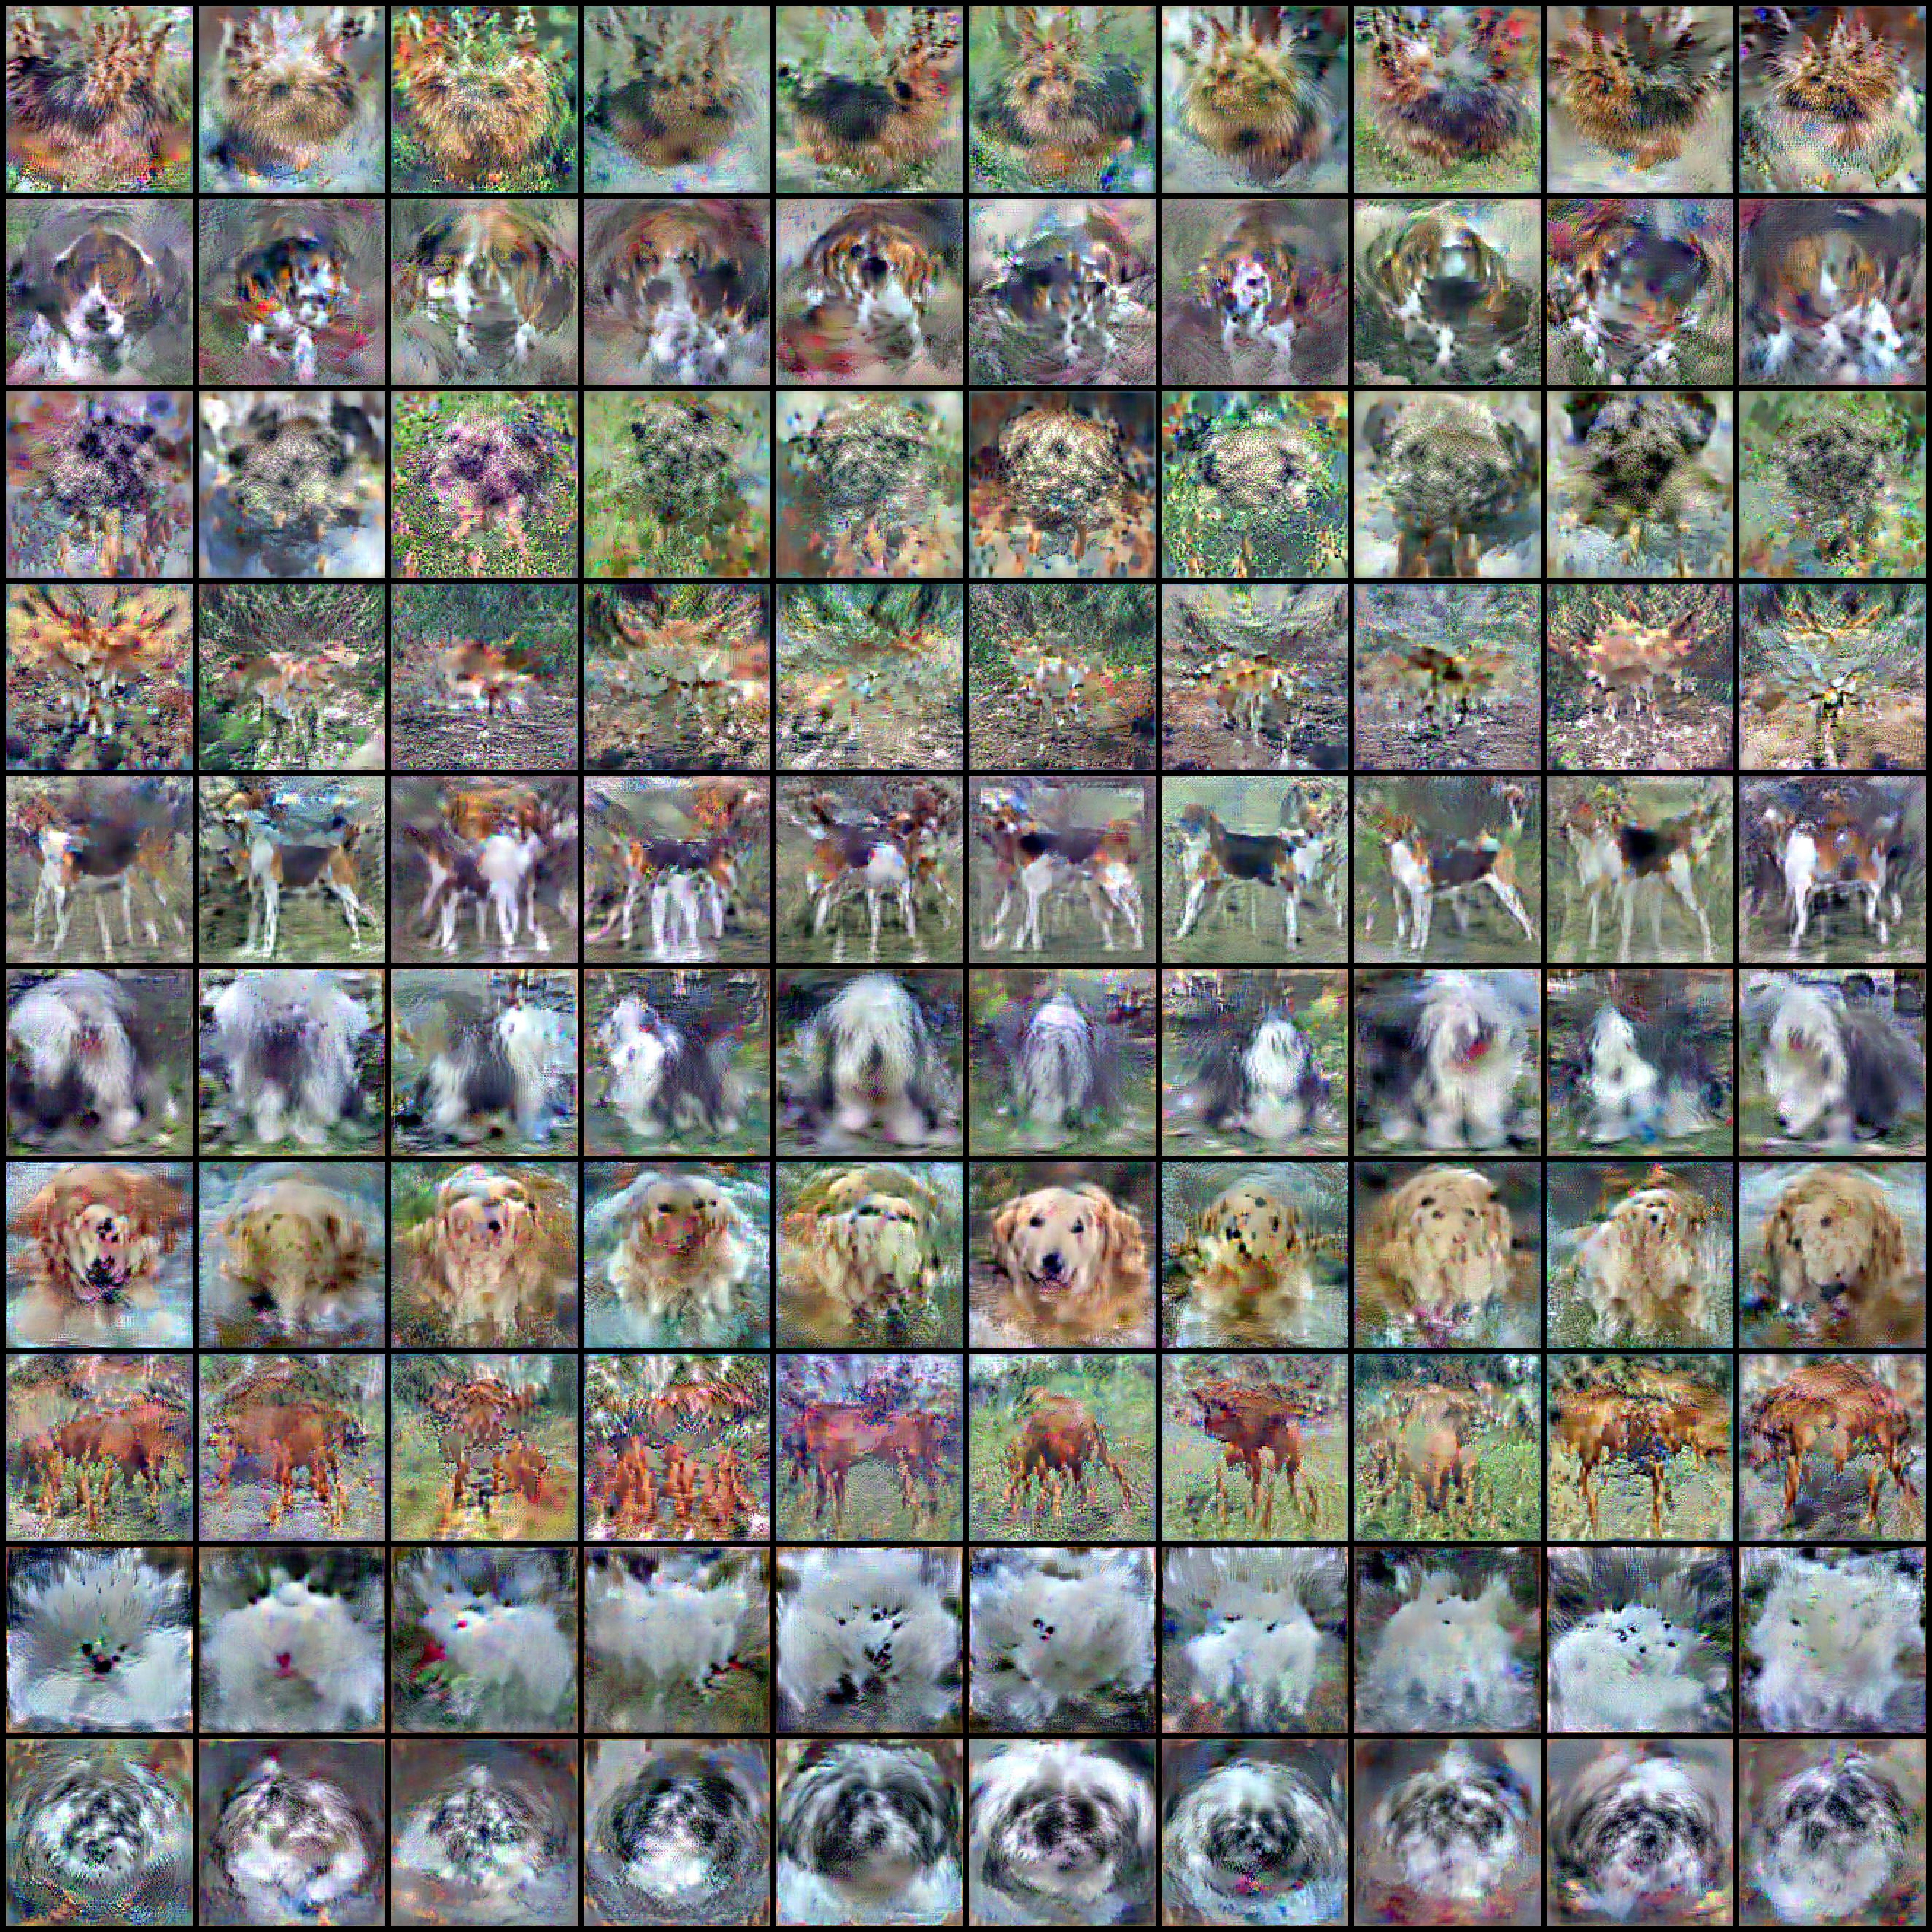
\includegraphics[width=\linewidth]{figures/imagenet_10/imagewoof_all.pdf}
    \caption{ImageWoof, 10 Images Per Class}
    \label{fig:woof_10}
\end{figure*}
\begin{figure*}
    \centering
    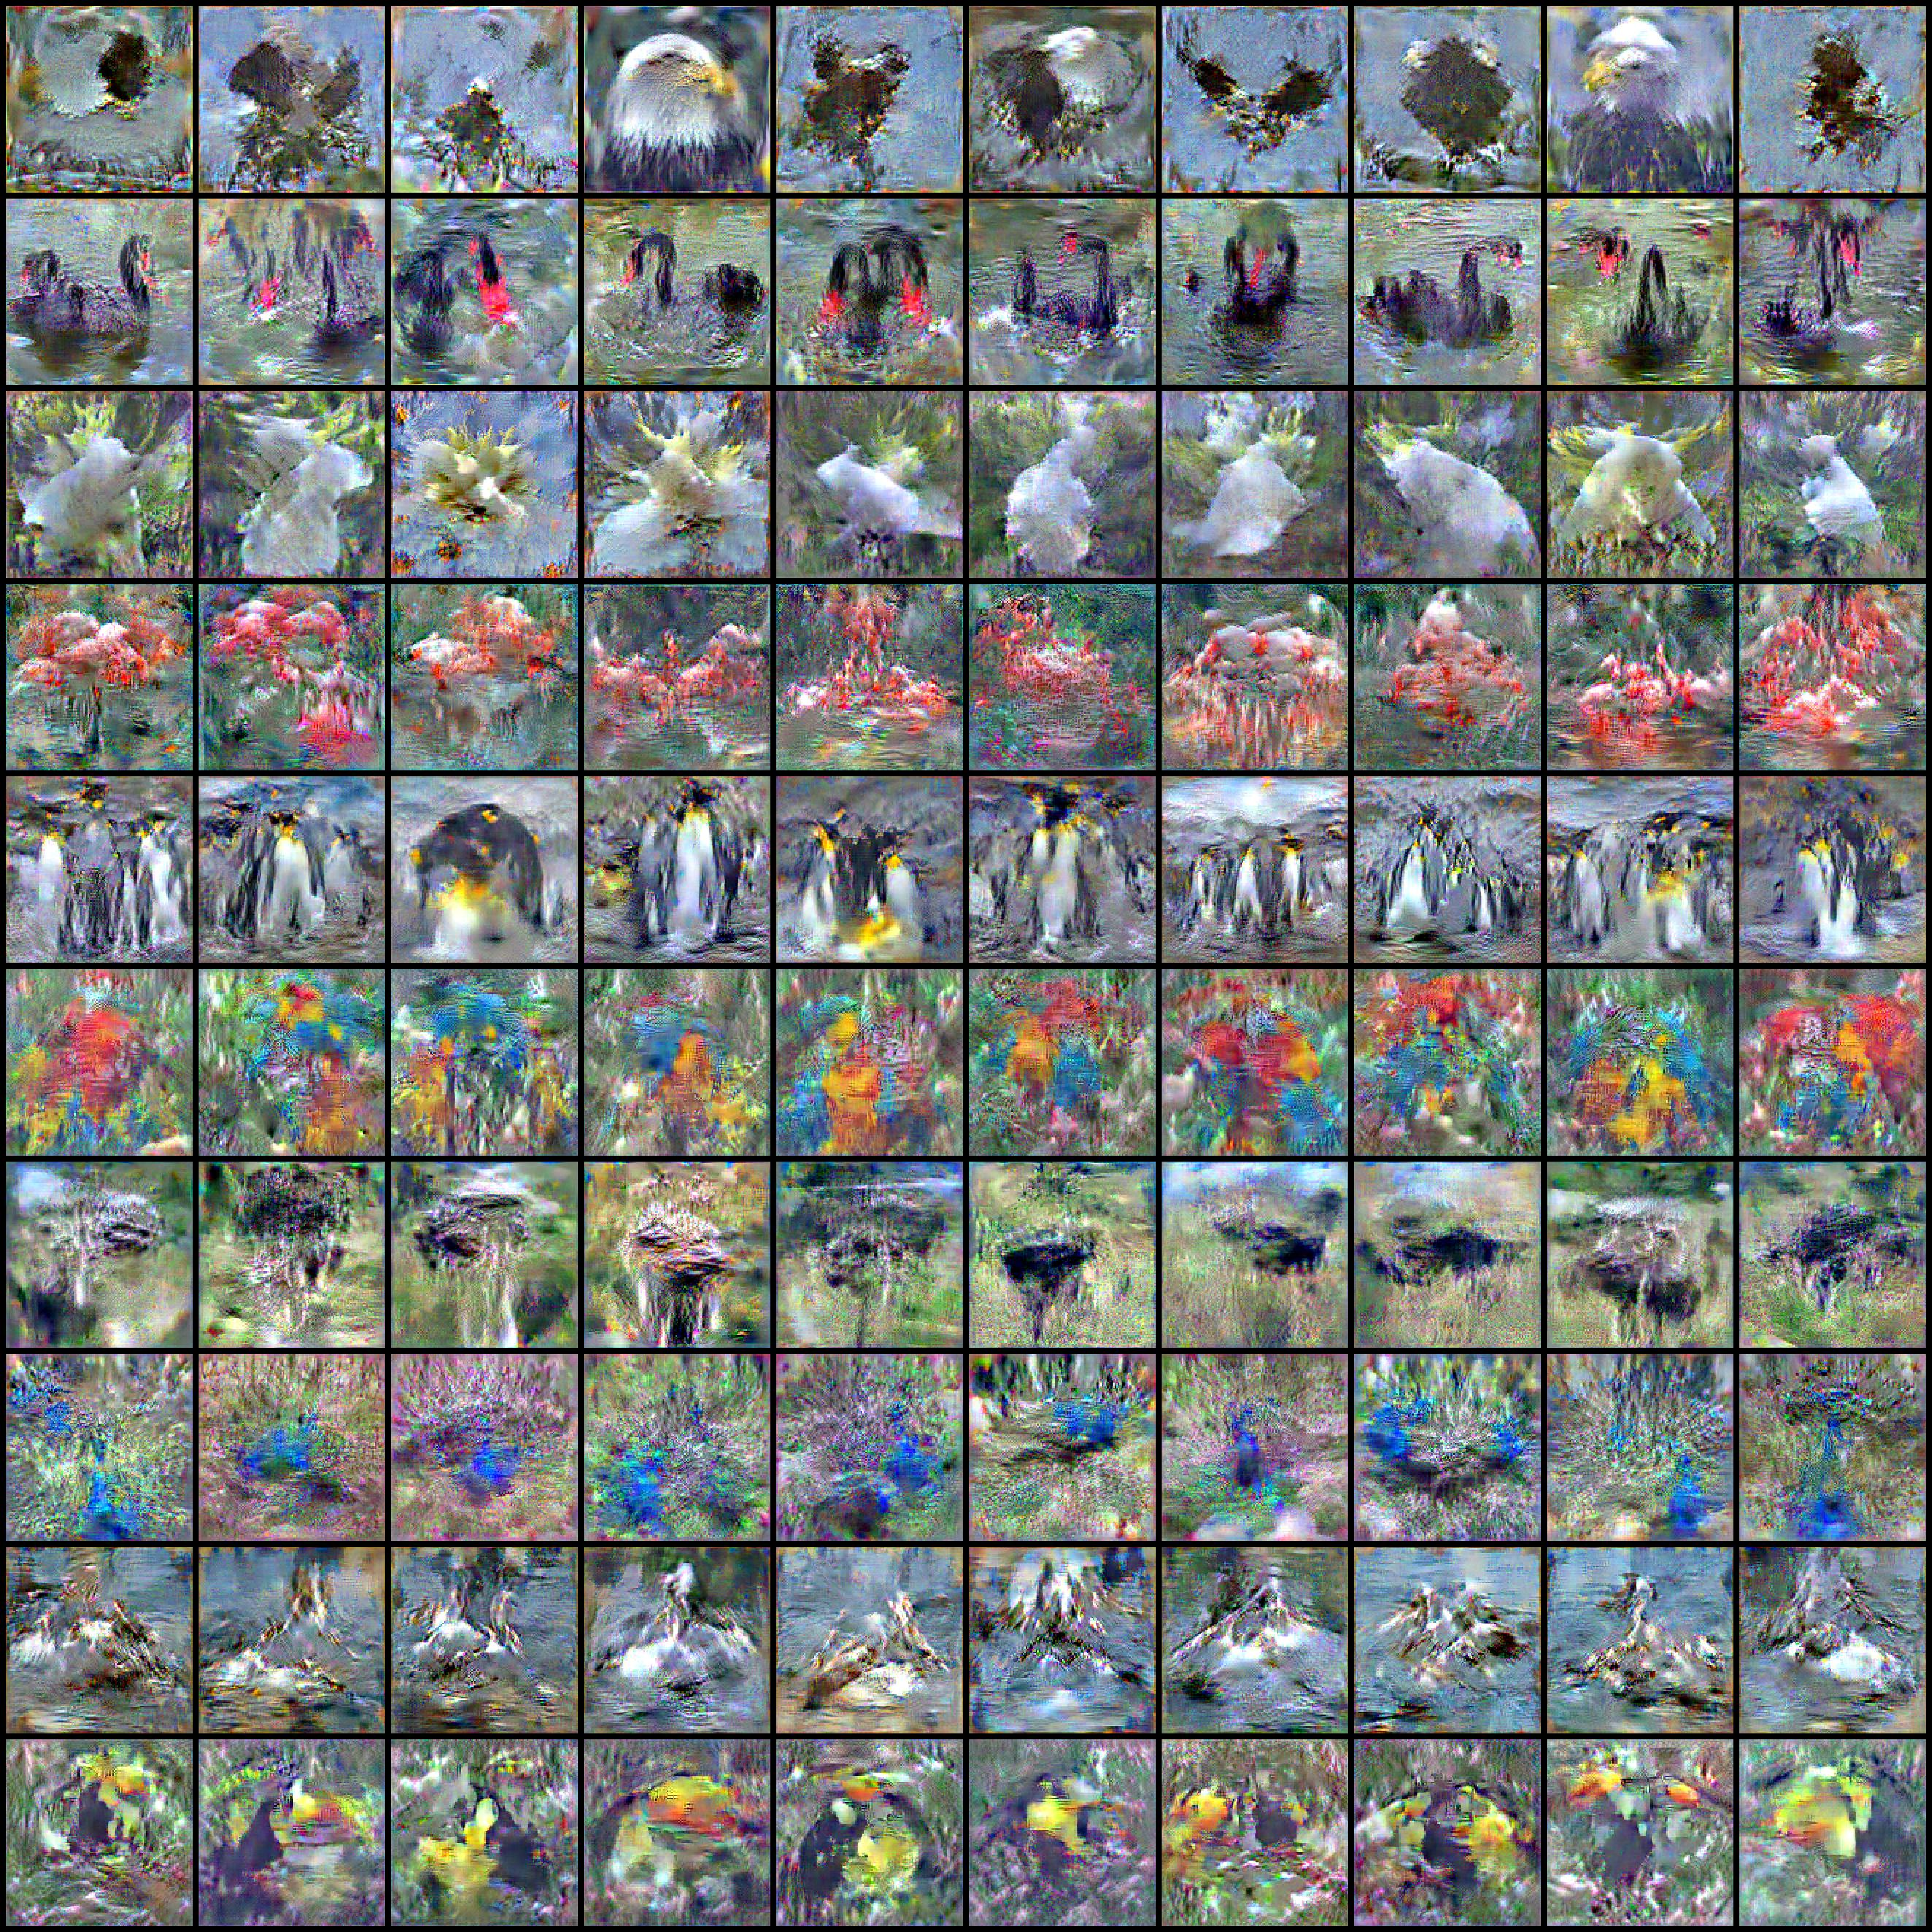
\includegraphics[width=\linewidth]{figures/imagenet_10/imagesquawk_all.pdf}
    \caption{ImageSquawk, 10 Images Per Class}
    \label{fig:squawk_10}
\end{figure*}
\begin{figure*}
    \centering
    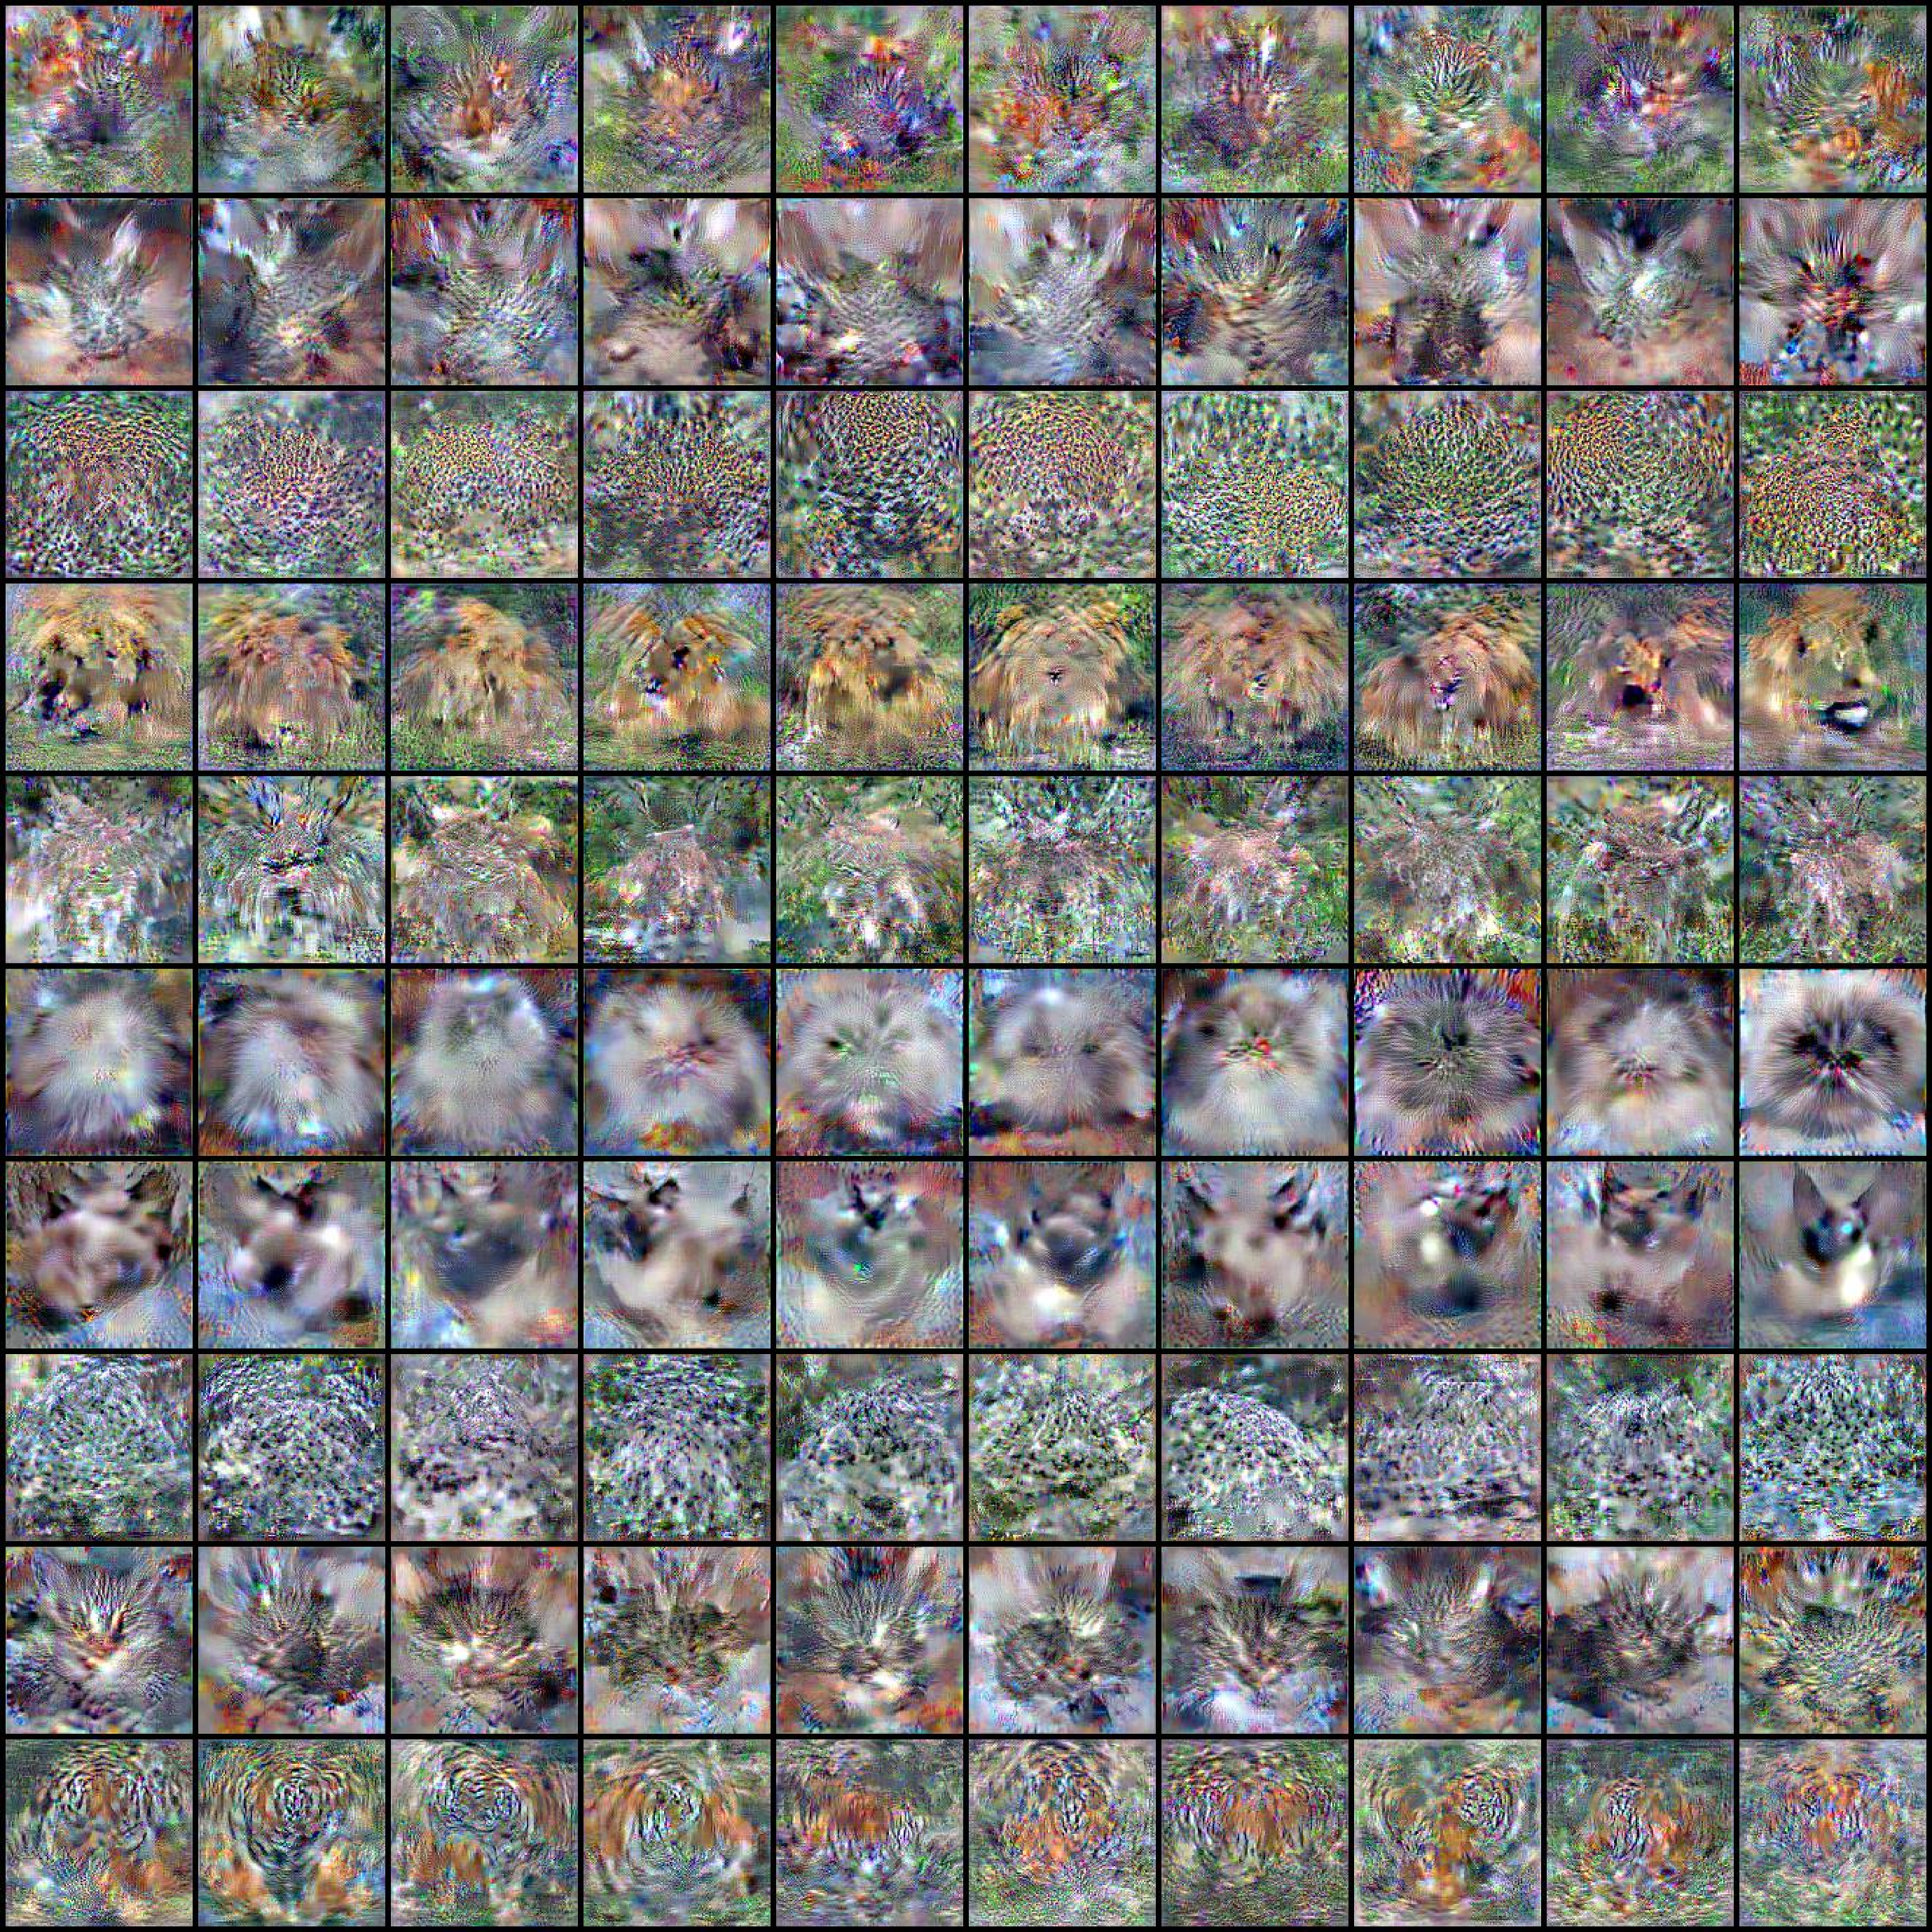
\includegraphics[width=\linewidth]{figures/imagenet_10/imagemeow_all.pdf}
    \caption{ImageMeow, 10 Images Per Class}
    \label{fig:meow_10}
\end{figure*}
\begin{figure*}
    \centering
    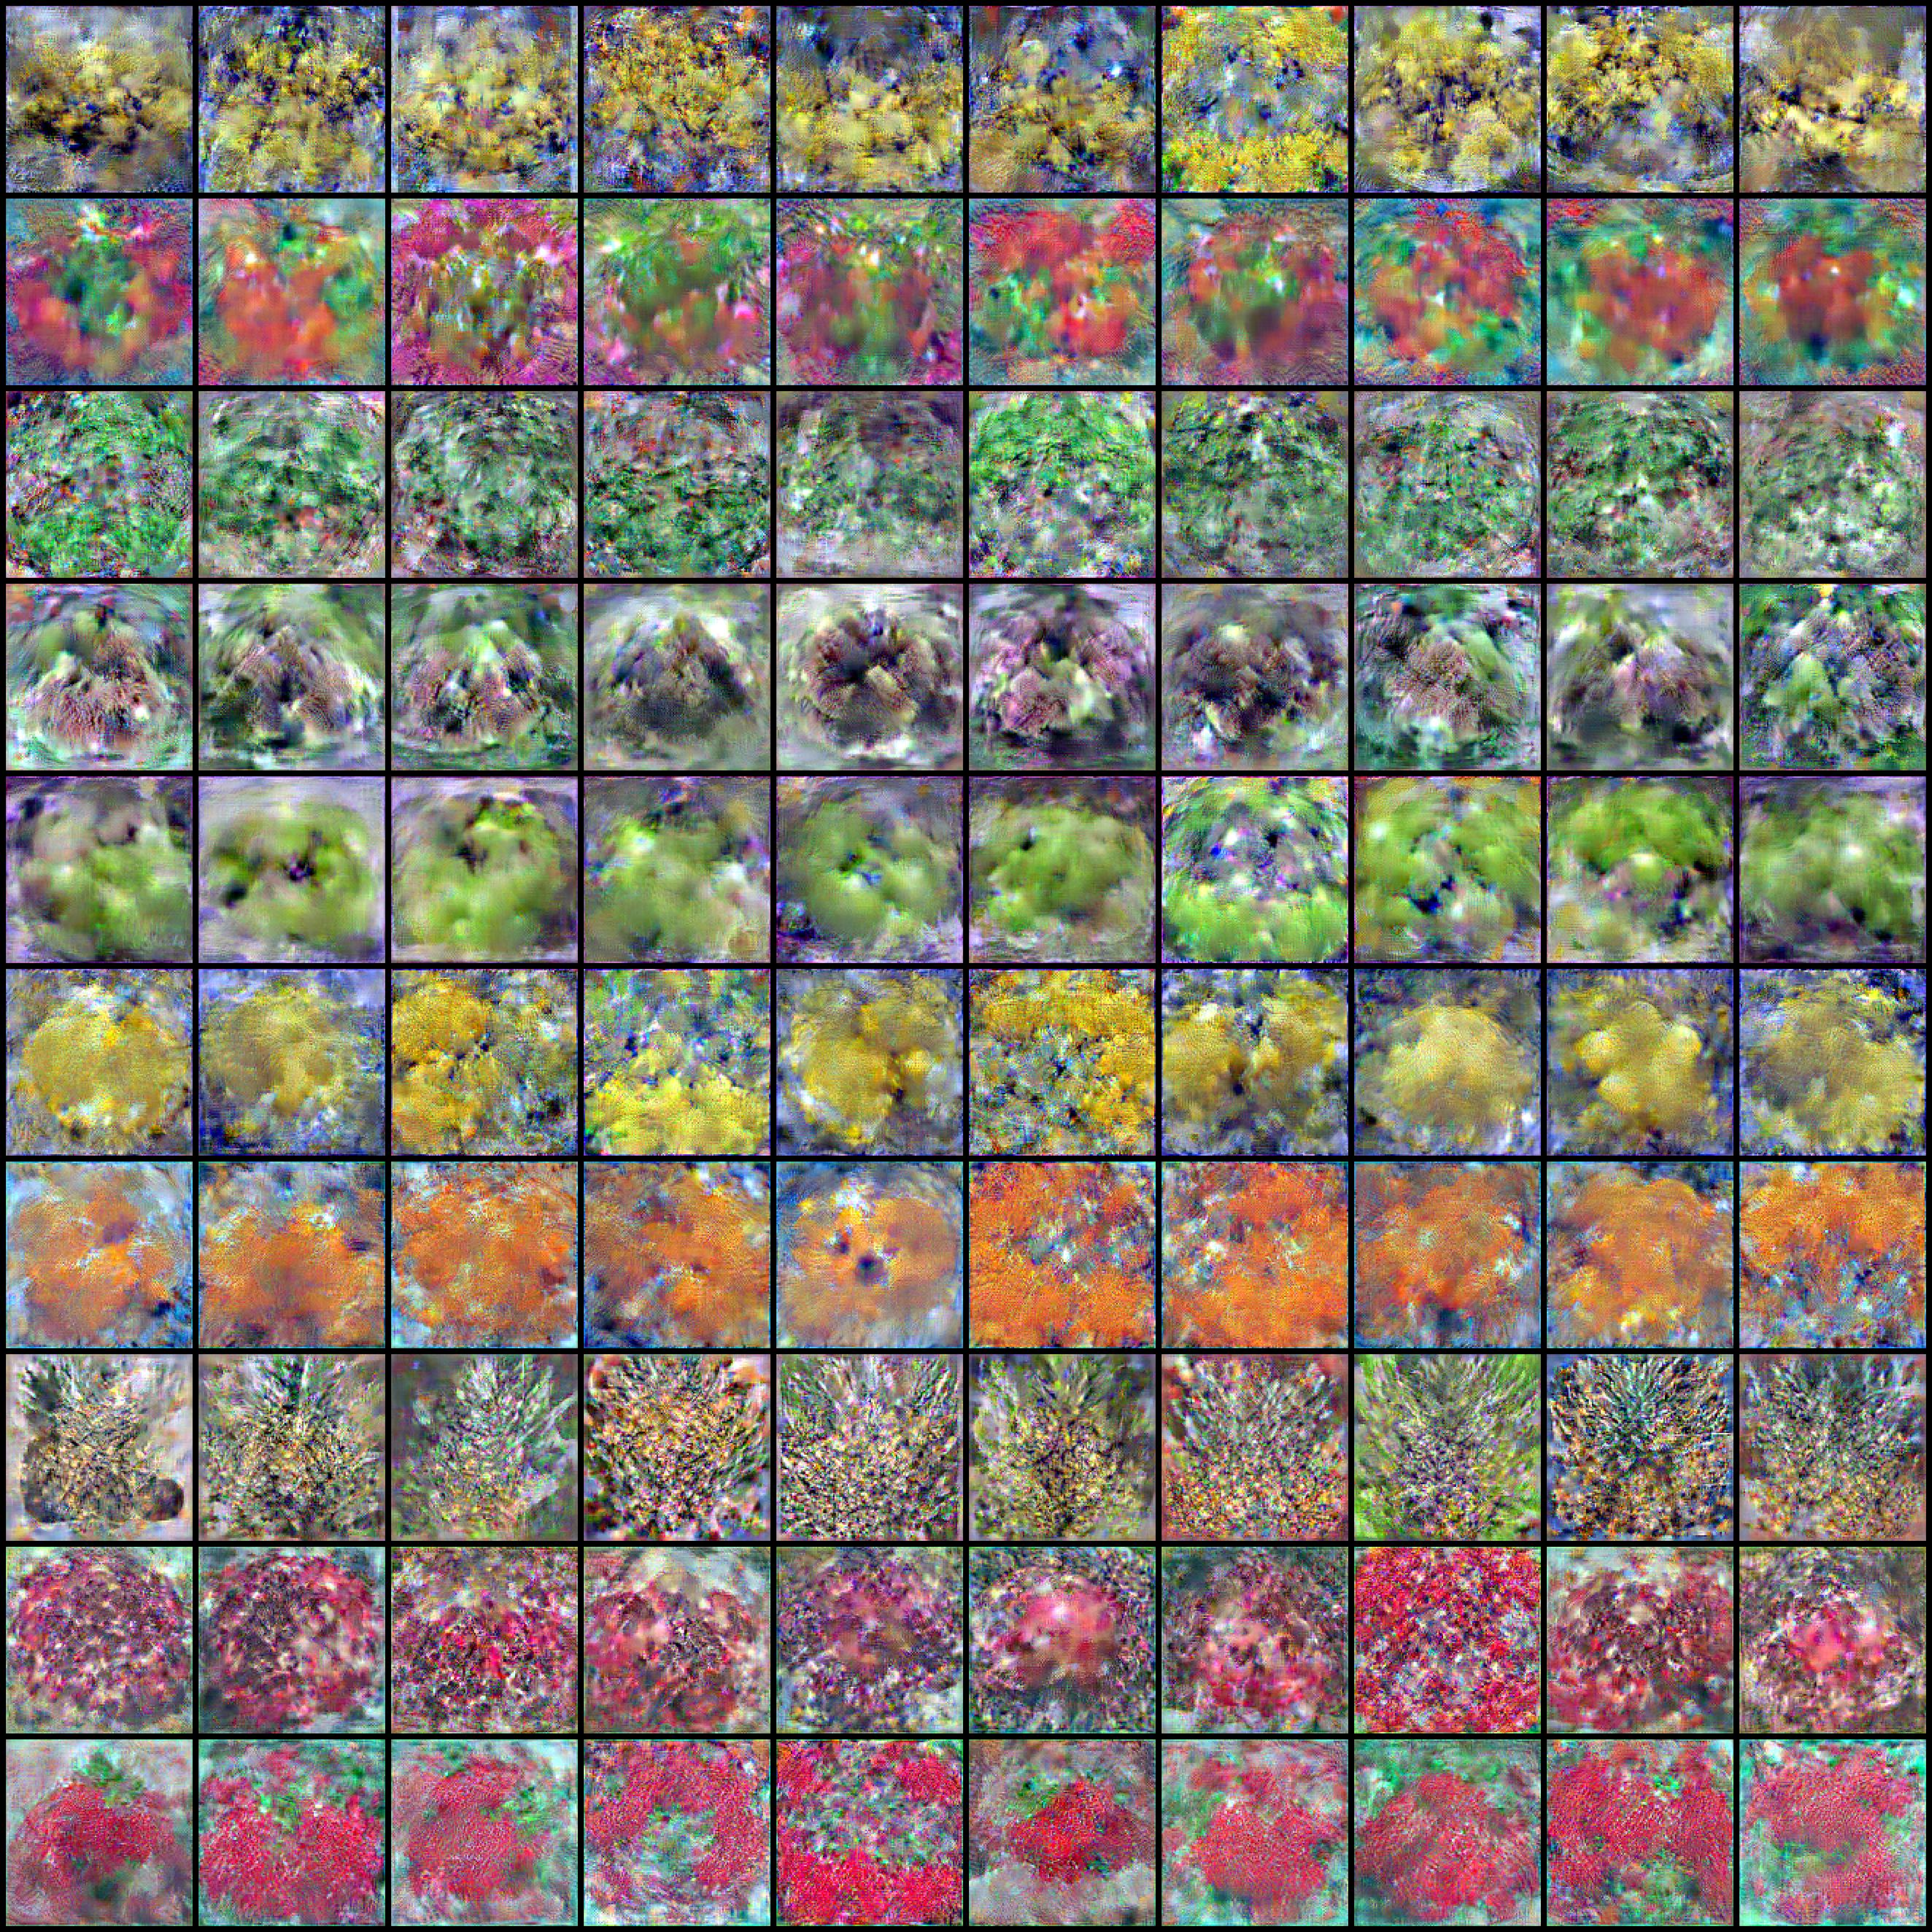
\includegraphics[width=\linewidth]{figures/imagenet_10/imagefruit_all.pdf}
    \caption{ImageFruit, 10 Images Per Class}
    \label{fig:fruit_10}
\end{figure*}
\begin{figure*}
    \centering
    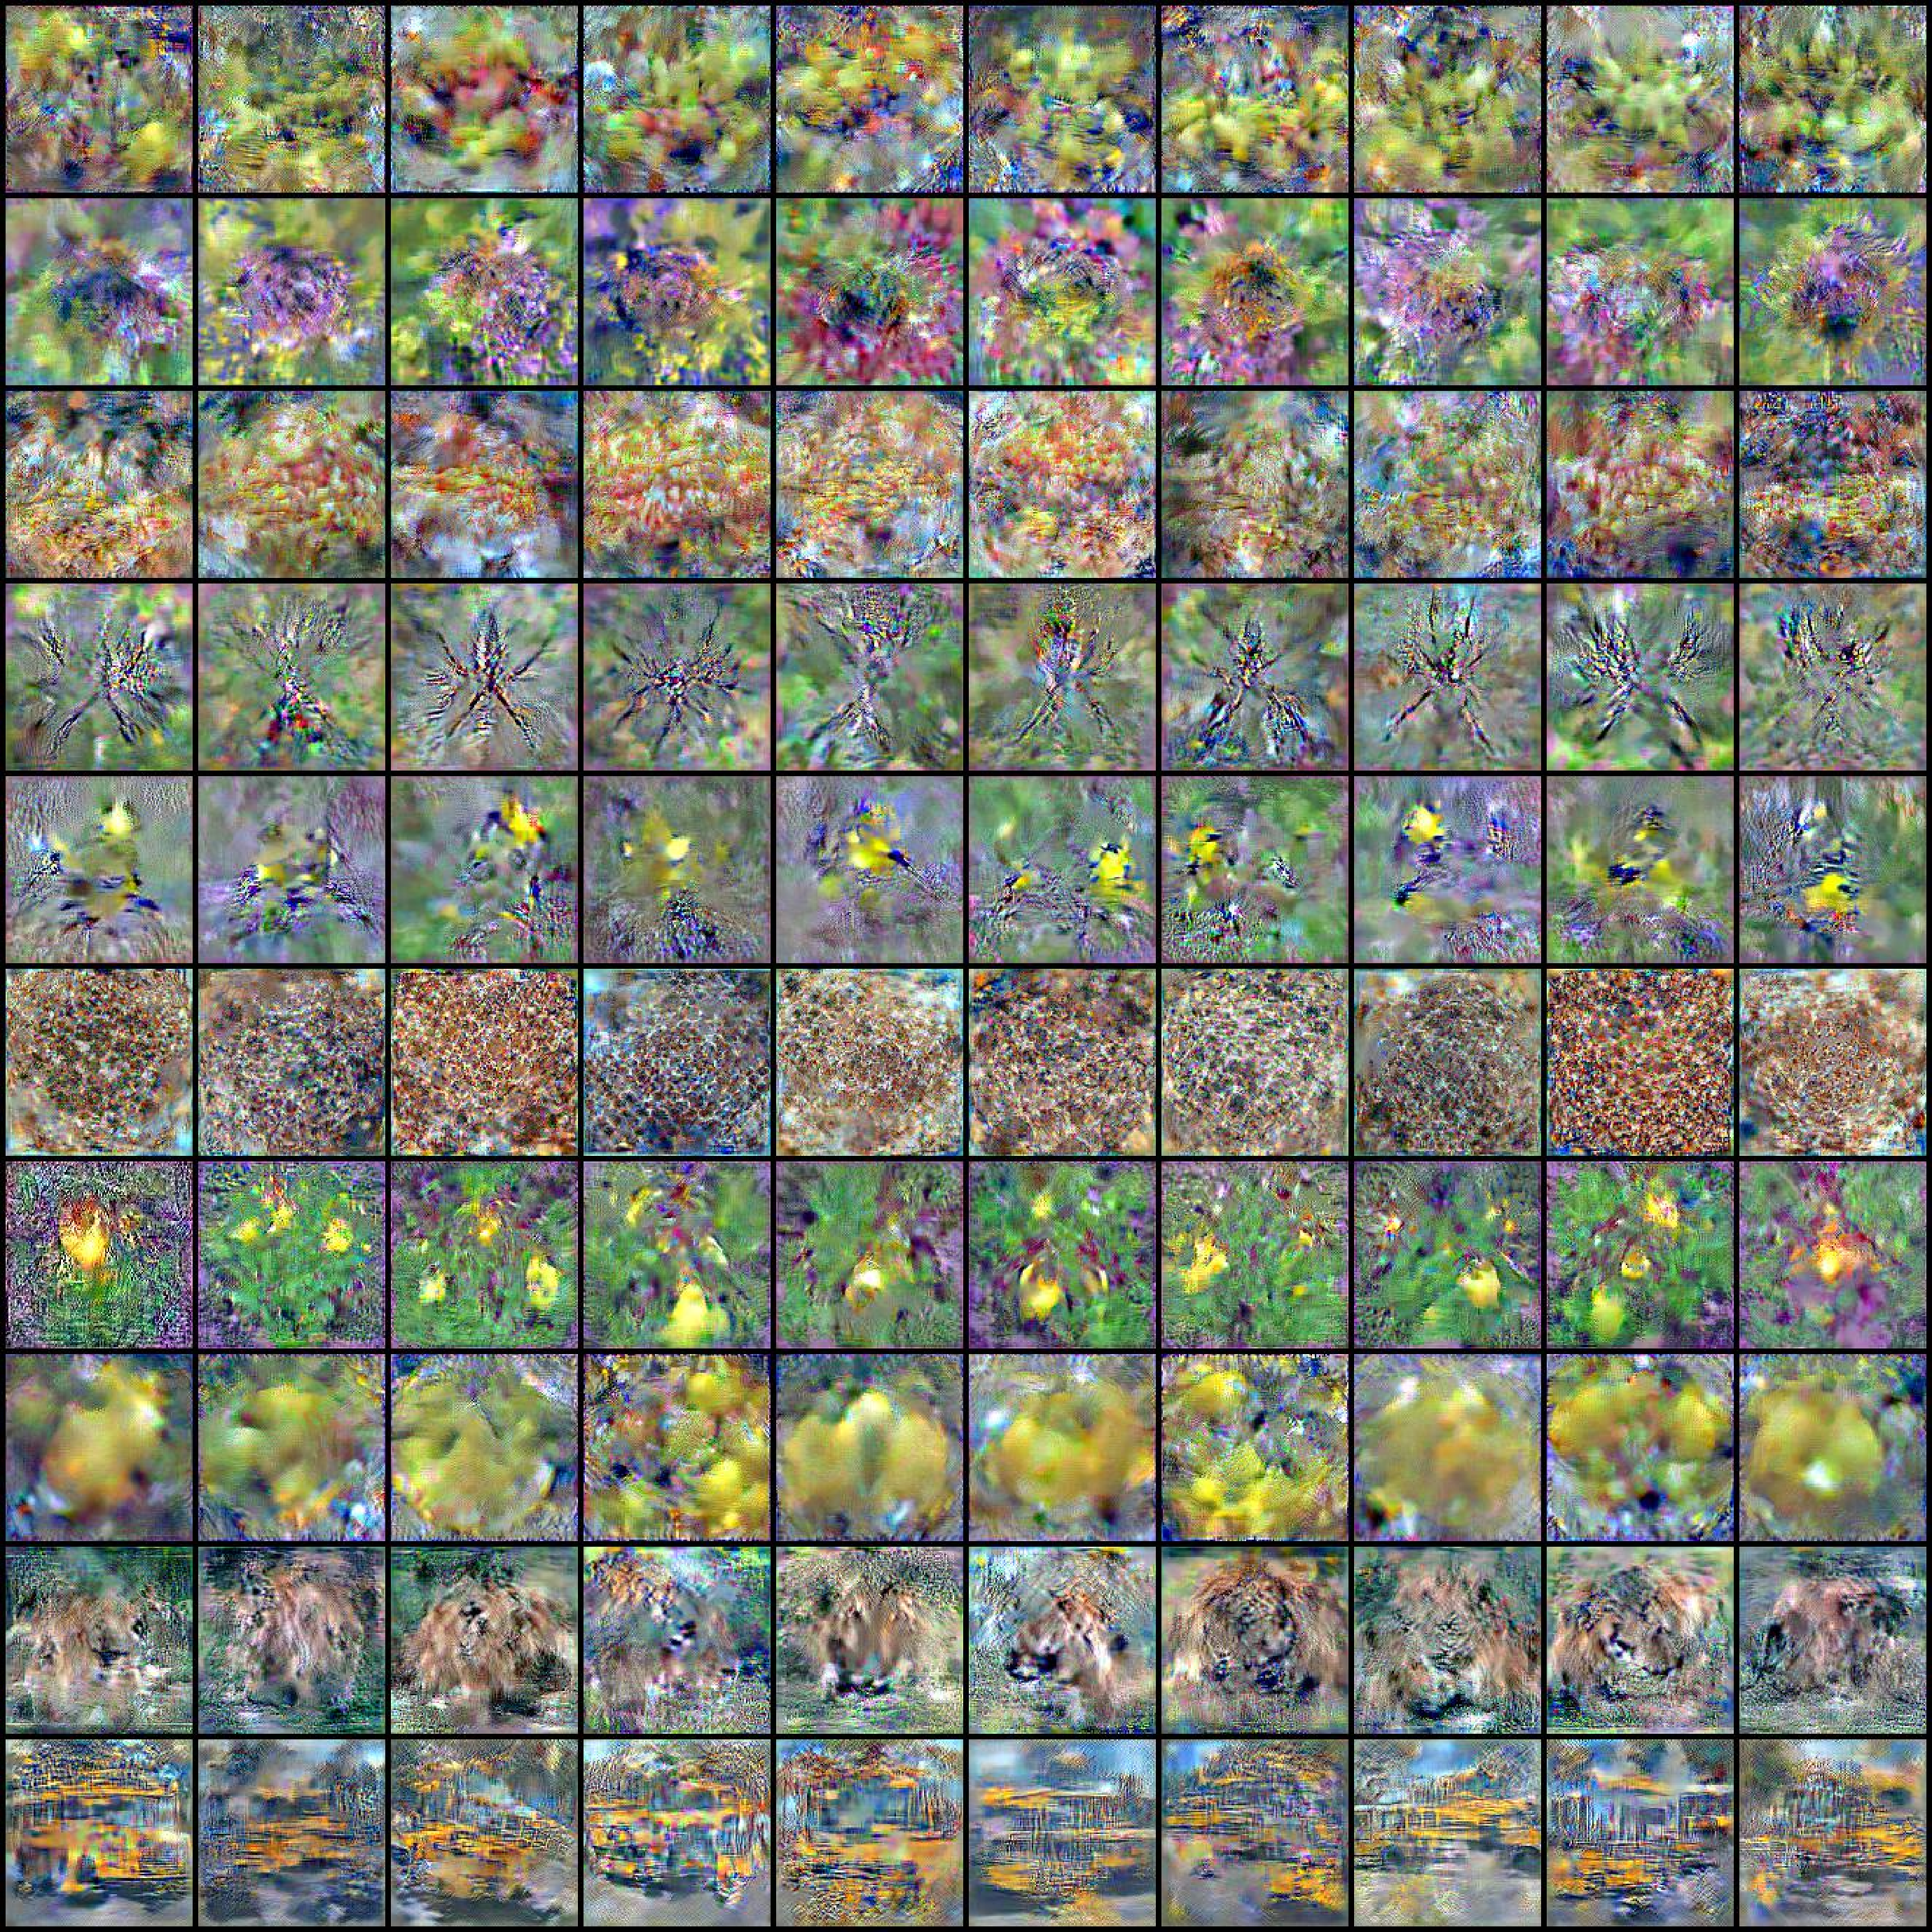
\includegraphics[width=\linewidth]{figures/imagenet_10/imageyellow_all.pdf}
    \caption{ImageYellow, 10 Images Per Class}
    \label{fig:yellow_10}
\end{figure*}
\vfill\break